\documentclass[10pt, journal, a4paper, twocolumn]{article}

%% ===== PACKAGES =====
\usepackage[utf8]{inputenc}
\usepackage{amsmath, amssymb, amsfonts}
\usepackage{graphicx}
\usepackage{booktabs} % Professional tables
\usepackage{tabularx} % Flexible width tables
\usepackage{multirow}
\usepackage{geometry} % Margins
\usepackage{authblk}  % Author block
\usepackage{xcolor}   % Colors
\usepackage{cite}     % Citation management
\usepackage{longtable} % Support for long tables in appendix
\usepackage{caption}
\usepackage{subcaption}
\usepackage{float}
\usepackage{titlesec} % Section formatting
\usepackage{microtype} % Optimization for spacing
\usepackage{tikz} % Used for drawing placeholder figures if images are missing

% Hyperref usually should be loaded last
\usepackage{hyperref} 

%% ===== GEOMETRY =====
\geometry{
 left=15mm,
 right=15mm,
 top=20mm,
 bottom=20mm,
 columnsep=6mm
}

%% ===== CUSTOM MACROS =====
\newcommand{\modelname}{\textbf{PACE-Former}}
\newcommand{\vopeak}{VO\textsubscript{2peak}}
\newcommand{\voat}{VO\textsubscript{2}@AT}
\newcommand{\dotve}{\(\dot{V}_E\)}
\newcommand{\dotvo}{\(\dot{V}O_2\)}
\newcommand{\dotvco}{\(\dot{V}CO_2\)}

%% ===== TITLE & AUTHORS =====
\title{\huge \textbf{\modelname: Bridging Clinical Safety and Diagnostic Precision in Multi-Center CPET via Systemic Style Adaptation}}

\author[1]{Cong Wang}
\author[2]{Bei Xu}
\author[1]{Shou-ling Mi\thanks{Corresponding author: email@address.com}}

\affil[1]{Zhongshan Hospital, Fudan University, Shanghai, China}
\affil[2]{BexiMed Co., Ltd., Shanghai, China}

\date{}

%% ===== BEGIN DOCUMENT =====
\begin{document}

\twocolumn[
  \begin{@twocolumnfalse}
    \maketitle
    \begin{abstract}
      \noindent \textbf{Background:} Cardiopulmonary exercise testing (CPET) is the gold standard for assessing cardiorespiratory fitness. However, its clinical deployment faces three critical challenges: physical heterogeneity across multi-center devices, the non-stationary nature of physiological signals, and safety risks during maximal testing in high-risk patients. Existing AI models focus primarily on offline retrospective analysis, failing to address the urgent clinical need for real-time safety monitoring and prognostic assessment.
      
      \noindent \textbf{Methods:} We propose Physiological Adaptive CPET Engine (\modelname), a unified framework utilizing a three-fold decoupling paradigm. (1) \textbf{Feature Decoupling:} An input-driven Style Encoder extracts ``systemic fingerprints'' from resting-phase data, using Conditional Layer Normalization to dynamically calibrate the network against holistic systemic heterogeneity (including variations in device physics, environmental conditions, and population demographics). (2) \textbf{Spatiotemporal Decoupling:} A hybrid masking training strategy enables a single model to perform both ``online causal inference'' (for low false-alarm rates) and ``offline global review'' (for high precision). (3) \textbf{Task Decoupling:} A dual-head architecture jointly outputs Anaerobic Threshold (AT) probability for diagnosis and scalar \vopeak{} prediction for prognosis, enabling ``Virtual Maximal Testing.''
      
      \noindent \textbf{Results:} Validated on a large-scale multi-center cohort ($N=14,036$) using 10-second aggregated data, the model achieved clinical-grade diagnostic precision in offline mode (Hit Rate within $\pm$20s $>$ 90\%). In online mode, it maintained an Early Trigger Rate $<$ 2\% while accurately predicting final \vopeak{} with $<$ 5\% error at 75\% test completion.
      
      \noindent \textbf{Conclusion:} \modelname{} successfully bridges the gap between clinical safety and diagnostic precision, offering a robust, generalized solution for intelligent CPET interpretation.
      
      \vspace{1em}
      \noindent \textbf{Keywords:} Cardiopulmonary Exercise Testing, Anaerobic Threshold, Time Series Forecasting, Domain Generalization, Virtual Maximal Testing
      \vspace{1em}
    \end{abstract}
  \end{@twocolumnfalse}
]

\section{Introduction}

\subsection{Background and Motivation}
Cardiopulmonary exercise testing (CPET) provides a holistic assessment of the cardiovascular, respiratory, and muscular systems. The Anaerobic Threshold (AT) and Peak Oxygen Uptake (\vopeak{}) derived from CPET are critical biomarkers for risk stratification in heart failure, perioperative assessment, and rehabilitation prescription.

However, the widespread clinical adoption of CPET AI faces distinct challenges compared to other medical domains. While breakthroughs in medical AI have focused on Anatomical Structural Recognition (e.g., lung nodule detection in CT), CPET analysis represents a higher-order challenge of Physiological Dynamics Inference. This task involves inherent epistemic uncertainty: AT is a metabolic phase transition occurring within muscle cells, invisible to direct observation. Models must solve a complex inverse problem to infer this moment from noisy, lagged gas exchange signals collected at the mouth. Furthermore, the ``ground truth'' for AT relies on expert interpretation of multi-dimensional curves, suffering from inherent inter-observer variability ($\approx \pm 30$s).

\subsection{The Data Challenge: Physiological Complexity and Signal Uncertainty}
Unlike standardized DICOM images or static disease classification tasks, CPET data represents a dynamic ``stress test'' of the human body, introducing unique physiological barriers to automated analysis:

\begin{itemize}
    \item \textbf{Heterophasic Coupling (The Synchronization Barrier):} Clinically, the ``truth'' of Anaerobic Threshold (AT) occurs in the muscle cells, but sensors measure the response at the mouth. This introduces a variable Circulatory Transit Delay—the time required for metabolite-rich blood to travel from muscle to lung. Crucially, this delay is pathology-dependent: a heart failure patient with low cardiac output exhibits a significantly longer lag (e.g., 40s) than a healthy athlete (e.g., 15s). Consequently, the metabolic ``cause'' (\dotvco{} rise) and the ventilatory ``effect'' (\dotve{} compensation) are asynchronously coupled. Models must learn to dynamically align these time-lagged physiological cues across diverse disease states, rather than assuming fixed temporal relationships.
    
    \item \textbf{Non-stationary Evolution (The Baseline Drift):} CPET is inherently a study of physiological flux. A patient transitions through distinct metabolic states—from rest, to aerobic exercise, to isocapnic buffering, and finally to respiratory decompensation. There is no static ``normal'': a heart rate of 110 bpm may be a baseline for one patient but a peak for another; a slope valid in the warm-up phase becomes pathological in the exercise phase. Algorithms cannot rely on spatial invariance (as in CNNs) but must capture transient phase transitions within a statistical distribution that drifts drastically from start to finish.
    
    \item \textbf{Stochastic Signal Volatility (The Noise-Information Conflict):} Breath-by-breath acquisition is physiologically ``noisy.'' Irregular breathing patterns (e.g., swallowing, coughing, or anxiety-induced hyperventilation) create high-frequency artifacts that mimic physiological inflection points. In clinical practice, experts visually ``filter'' these out based on context. For AI, this creates a sensitivity-stability conflict: excessive smoothing obliterates the sharp ``V-slope'' inflection required for precise AT localization, while raw processing leaves the model vulnerable to triggering on transient artifacts rather than true metabolic shifts.
\end{itemize}

\subsection{The Clinical Dilemma: Safety vs. Precision}
Current single-task models fail to reconcile the contradictory objectives inherent in real-world clinical workflows, creating a deployment deadlock rooted in the data challenges described above:

\begin{itemize}
    \item \textbf{Online Monitoring (The Safety Imperative):} For high-risk populations (e.g., severe heart failure), the priority is immediate risk aversion. Clinicians need a ``Virtual Maximal Test'' to predict endpoints early and terminate the test before actual exhaustion. The dilemma here is the Zero-Tolerance for False Alarms: To ensure safety, the model must react instantaneously to physiological limits; yet to avoid ``wasting'' a test due to premature termination (false positives) caused by signal artifacts, it must be conservative. This creates a ``hesitancy gap''—current models are either too unstable to complete a test or too slow to prevent adverse events.
    
    \item \textbf{Offline Reporting (The Accessibility-Precision Gap):} Post-test diagnosis faces a Resource-Accuracy Dilemma. CPET interpretation is a highly specialized skill with a steep learning curve, rendering it largely inaccessible in primary care. Even for specialists, manual interpretation is labor-intensive and time-consuming, severely limiting patient throughput. While AI automation is the logical solution to this bottleneck, current models fail to bridge the ``trust gap.'' Algorithms optimized for smooth online monitoring often sacrifice the granular signal fidelity required to pinpoint subtle metabolic transitions (AT), leaving clinicians with no choice but to rely on scarce, slow human expertise to guarantee diagnostic rigor.
\end{itemize}

\subsection{The Deployment Bottleneck: Systemic Heterogeneity \& Data Fragmentation}
A major barrier to multi-center deployment is the ``Holistic Systemic Heterogeneity'' unique to each clinical center, manifesting at both physical and infrastructural levels:

\begin{itemize}
    \item \textbf{The Physical Fingerprint:} Differences in hardware sensors (e.g., Ultrasonic vs. Turbine) and environmental physics create severe systemic time biases and signal drifts. Combined with the patient-specific non-stationarity (Section 1.2), this creates a compound domain shift that conventional models cannot generalize across.
    
    \item \textbf{The Infrastructural Chaos:} Clinical deployment is further paralyzed by a Fragmented Data Ecosystem. Even when disparate vendors (e.g., COSMED vs. Ganshorn) export to a common file format like .xlsx, they enforce mutually incompatible internal schemas. Divergent column taxonomies, inconsistent unit standards, and varying header structures create a ``semantic chasm'' between devices. This is compounded by wide variations in clinical protocols (e.g., Ramp rates, Warm-up durations). Without a unified standard, AI models are trapped in ``vendor lock-in,'' unable to scale across multi-center environments with heterogeneous device fleets.
\end{itemize}

\subsection{Our Contributions: Unifying the Divide via Three-Fold Decoupling}
To resolve the conflicting clinical mandates and physiological barriers described above, we propose the Physiological Adaptive CPET Engine (\modelname), a unified framework utilizing a novel Three-Fold Decoupling Paradigm:

\begin{itemize}
    \item \textbf{Spatiotemporal Decoupling (Solving the Hesitancy Gap):} We introduce a hybrid masking strategy combined with a Prognostic Head. This enables ``Virtual Maximal Testing''—accurately predicting \vopeak{} at sub-maximal loads to ensure safety—while employing Causal Masking to eliminate the algorithmic lag inherent in traditional filters.
    
    \item \textbf{Global Contextualization (Solving the Trust Gap):} We propose a Bidirectional Attention mechanism for offline reporting. By integrating Recovery Phase dynamics, the model restores the granular signal fidelity lost in real-time monitoring, achieving expert-level diagnostic precision.
    
    \item \textbf{Feature Decoupling (Solving the Deployment Gap):} We design an Input-Driven Style Encoder and the CPETx Standardization Framework. Together, they decouple physiological signals from hardware-specific ``physical fingerprints'' and infrastructural chaos, enabling robust generalization across heterogeneous multi-center environments.
\end{itemize}

\section{Methodology}

The overall framework of \modelname{} is illustrated in Fig.~\ref{fig:arch}. The system is designed to handle the full lifecycle of CPET analysis, from heterogeneous data ingestion to dual-mode clinical inference. We organize this section as follows: Section \ref{sec:data_infra} introduces the CPETx infrastructure for harmonizing multi-center data. Section \ref{sec:model_arch} details the \modelname{} architecture, specifically the Style-Aware Backbone and Dual-Head design. Finally, Sections \ref{sec:training} and \ref{sec:loss} describe the Hybrid Training Strategy and Physiological Loss Functions that enable the simultaneous optimization of safety and precision.

\subsection{Data Infrastructure and Strategy}
\label{sec:data_infra}
\begin{figure*}[t]
    \centering
    % 请确保图片文件名一致
    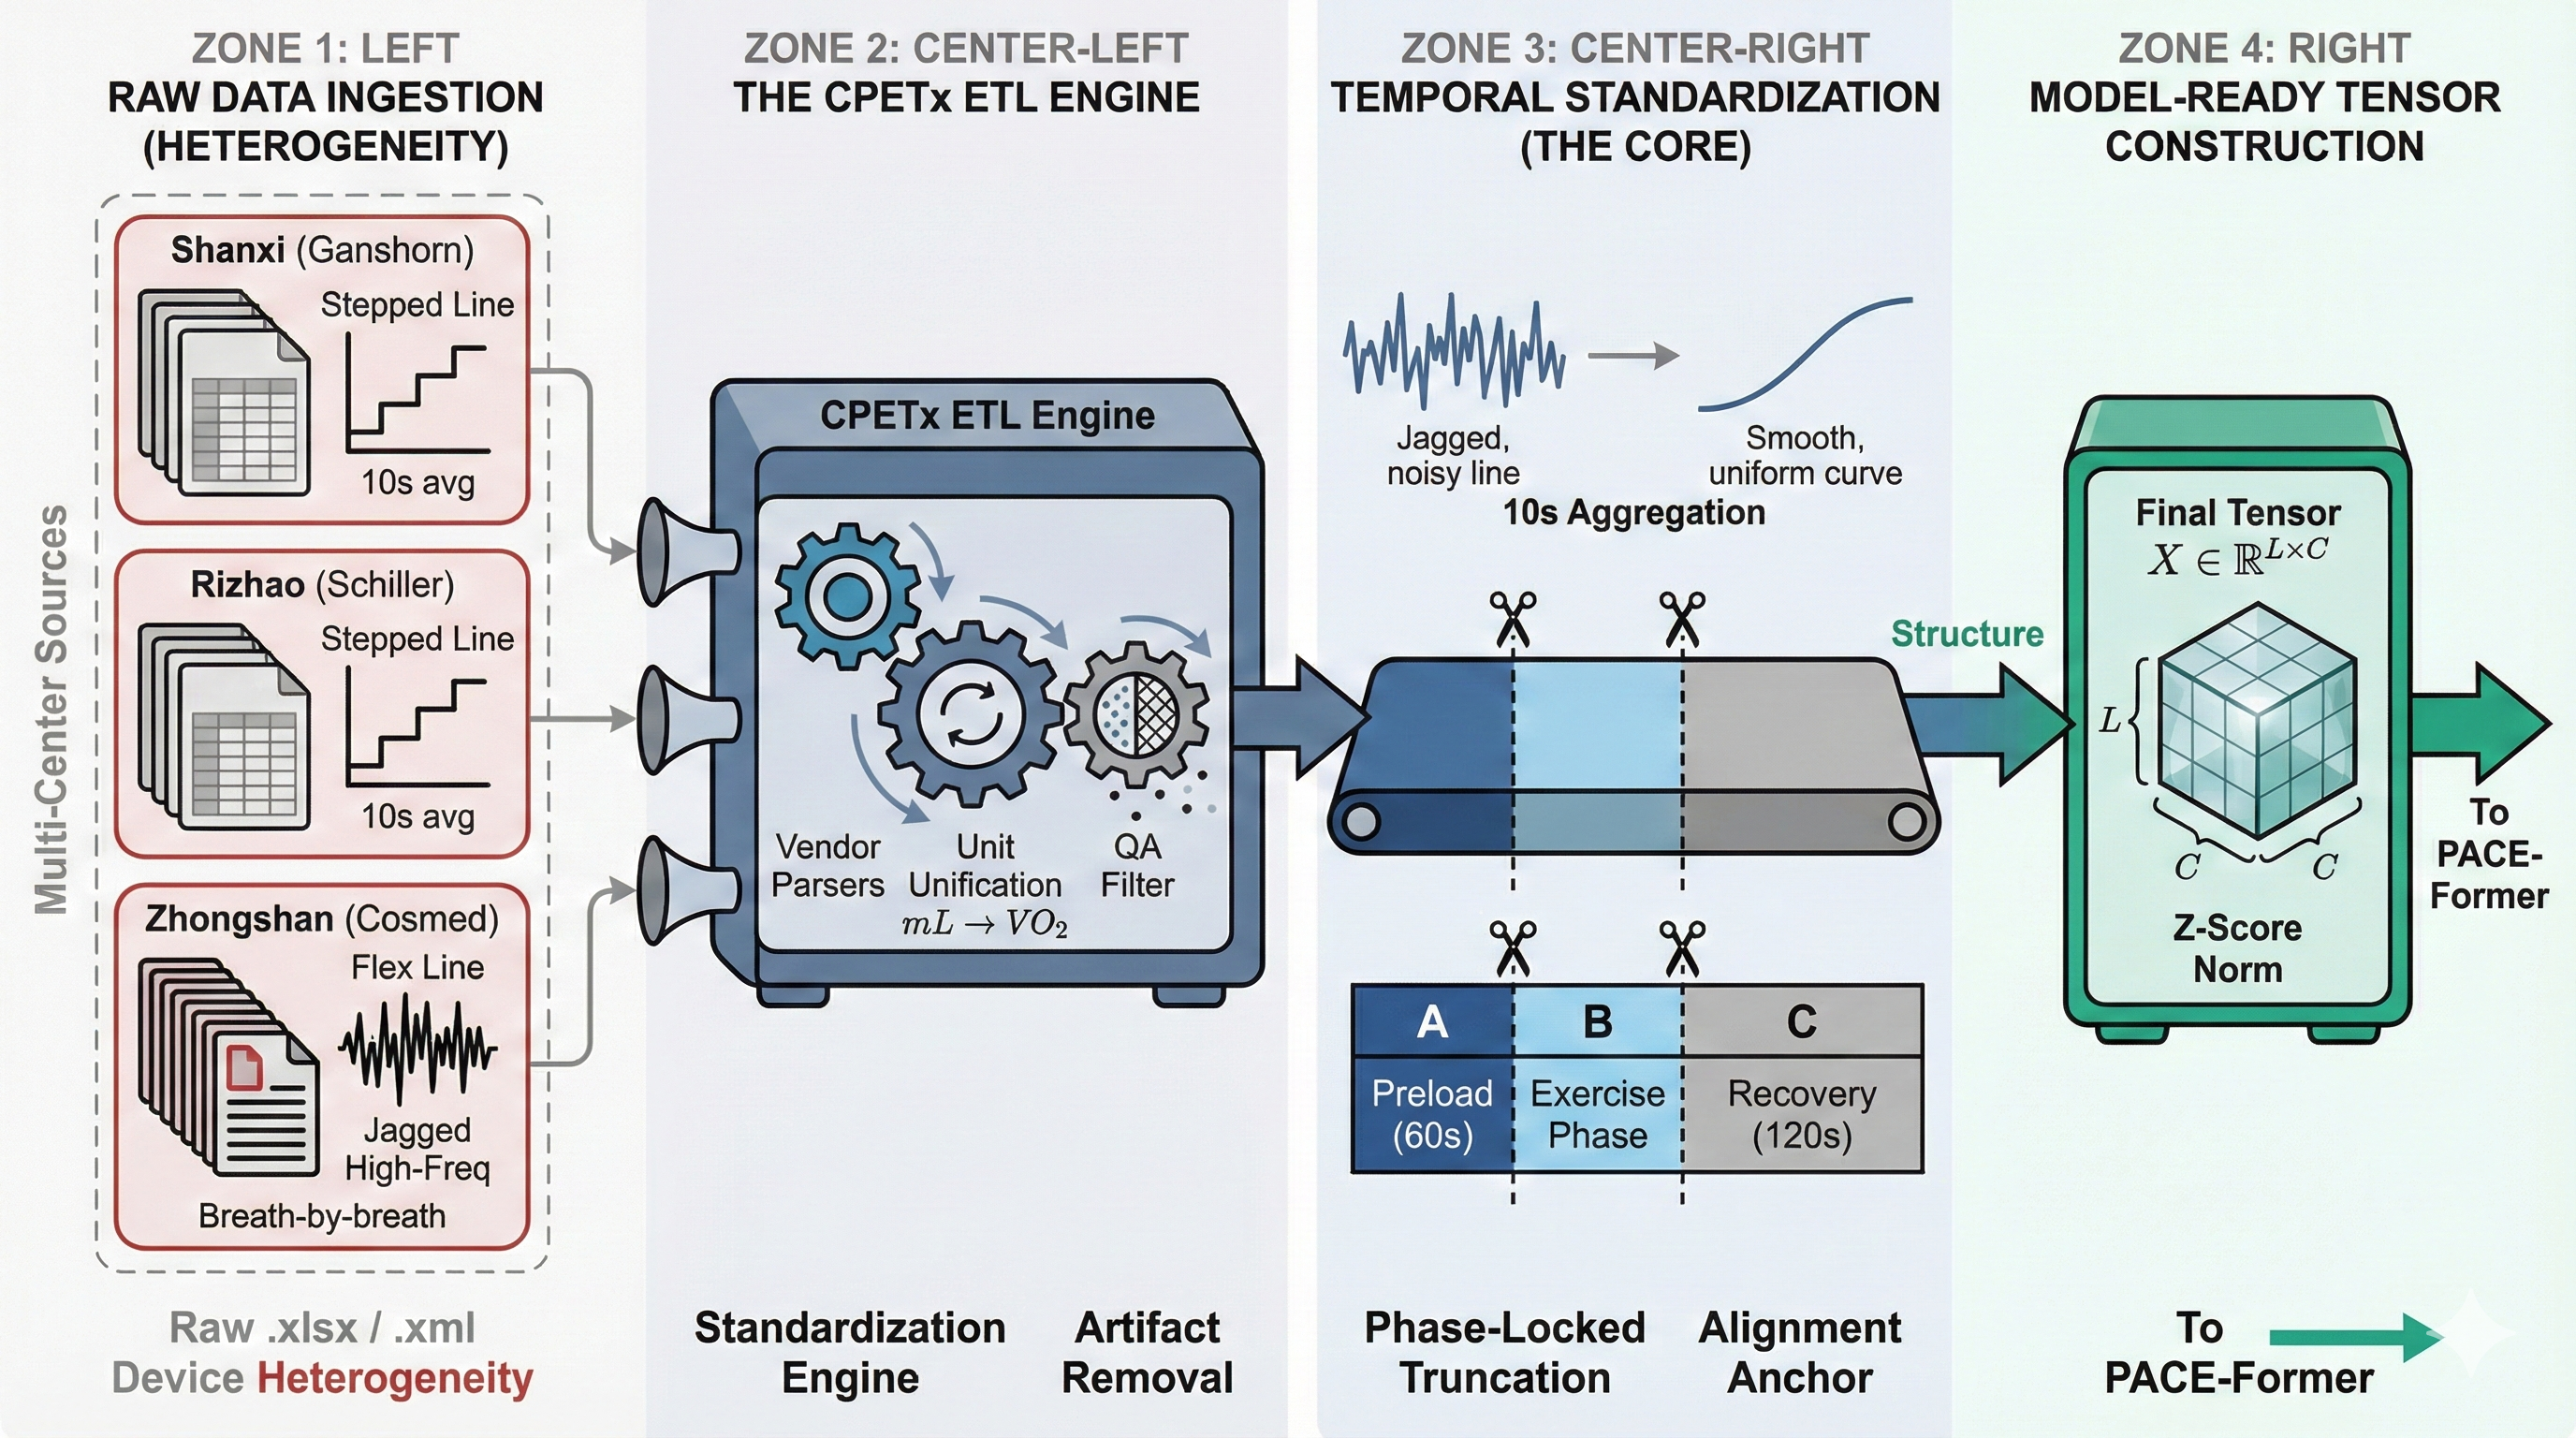
\includegraphics[width=\textwidth]{figures/data_flow.png}
    \caption{\textbf{The CPETx Data Standardization Pipeline.} Raw heterogeneous data from multi-center devices (Ganshorn, Cosmed) are ingested through vendor-specific parsers, mapped to a unified schema (CPETx), and transformed into aligned tensors via 10-second aggregation and phase-locked truncation.}
    \label{fig:data_pipeline}
\end{figure*}

\subsubsection{The CPETx Standardization Framework}
To address the challenge of device heterogeneity, we developed \textbf{CPETx}, a unified data schema and ingestion pipeline. This framework standardizes raw data from divergent proprietary schemas into a canonical representation. It resolves the critical issue of semantic heterogeneity, where disparate vendors (e.g., Ganshorn, COSMED) may utilize identical file extensions (e.g., .xlsx) yet enforce mutually incompatible internal structures.



The schema defines 70+ physiological variables, enforcing consistent units (e.g., $VO_2$ in mL/min, Pressure in mmHg) and data types. To automate the ingestion process, we developed a modular \textbf{Vendor-Agnostic Extraction Engine} that resolves proprietary format idiosyncrasies through three critical operations:
\begin{enumerate}
    \item \textbf{Fuzzy Mapping:} Employing regex-based matching to map diverse vendor taxonomies to the canonical CPETx variable space.
    \item \textbf{Phase Inference:} Parsing unstructured event markers to reconstruct the precise Load Phase trajectory (Rest/Exercise/Recovery).
    \item \textbf{Semantic Cleaning:} Sanitizing non-numeric artifacts and normalizing units.
\end{enumerate}
Crucially, the pipeline integrates a rigid Quality Control (QC) module that validates signal integrity during ingestion, automatically flagging files with structural corruption.

\subsubsection{Preprocessing: Physics-Aware Meso-scale Aggregation}
To resolve the sensitivity-stability conflict (Section 1.2) and harmonize sampling rates, we implemented a Physics-Aware Aggregation Module to transform breath-by-breath data into unified 10-second bins. Distinct statistical strategies were applied to preserve fidelity:
\begin{itemize}
    \item \textbf{Gas Exchange Volumetrics:} Calculated via Time-Weighted Averaging with Winsorization to suppress transient respiratory artifacts (e.g., coughs) without blunting the V-slope.
    \item \textbf{Derived Ratios (e.g., RER):} Re-computed as the Ratio of Aggregated Sums to strictly adhere to mass conservation laws.
    \item \textbf{Ergometric State:} Load parameters (Power, RPM) recorded using Last-Value Latching to accurately reflect target intensity.
\end{itemize}

\subsubsection{Temporal Alignment: Phase-Locked Tensor Construction}
To neutralize temporal heterogeneity caused by varying clinical protocols, we implemented a Phase-Locked Truncation strategy anchored to physiological state boundaries:
\begin{itemize}
    \item \textbf{Preload Context (Baseline Capture):} We retain a fixed window of 60 seconds (6 steps) preceding load onset. This captures the patient's resting baseline—essential for Style Encoder calibration.
    \item \textbf{Exercise Phase (Dynamic Capture):} The complete ramp exercise sequence is preserved intact.
    \item \textbf{Recovery Phase (Kinetic Capture):} We retain a fixed window of 120 seconds (12 steps) post-peak to capture immediate recovery kinetics without introducing ``shortcut learning.''
\end{itemize}
The resulting input tensor $X \in \mathbb{R}^{L \times C}$ consists of these concatenated segments, where $L = 6 + L_{load} + 12$.

\subsubsection{Normalization: Split-Aware Standardization}
To rigorously prevent data leakage, we discarded global normalization in favor of a Split-Aware Standardization strategy. Z-score statistics ($\mu, \sigma$) were computed exclusively on the training subset of each fold and frozen for application to validation/test sets. This ensures the model remains agnostic to test data distribution, simulating true clinical deployment.

\subsection{Model Architecture: The PACE-Former Framework}
\label{sec:model_arch}

As illustrated in Fig.~\ref{fig:arch}, the architecture maps heterophasic physiological inputs into simultaneous diagnostic probabilities and prognostic values using three physically-grounded modules.

\begin{figure*}[t]
    \centering
    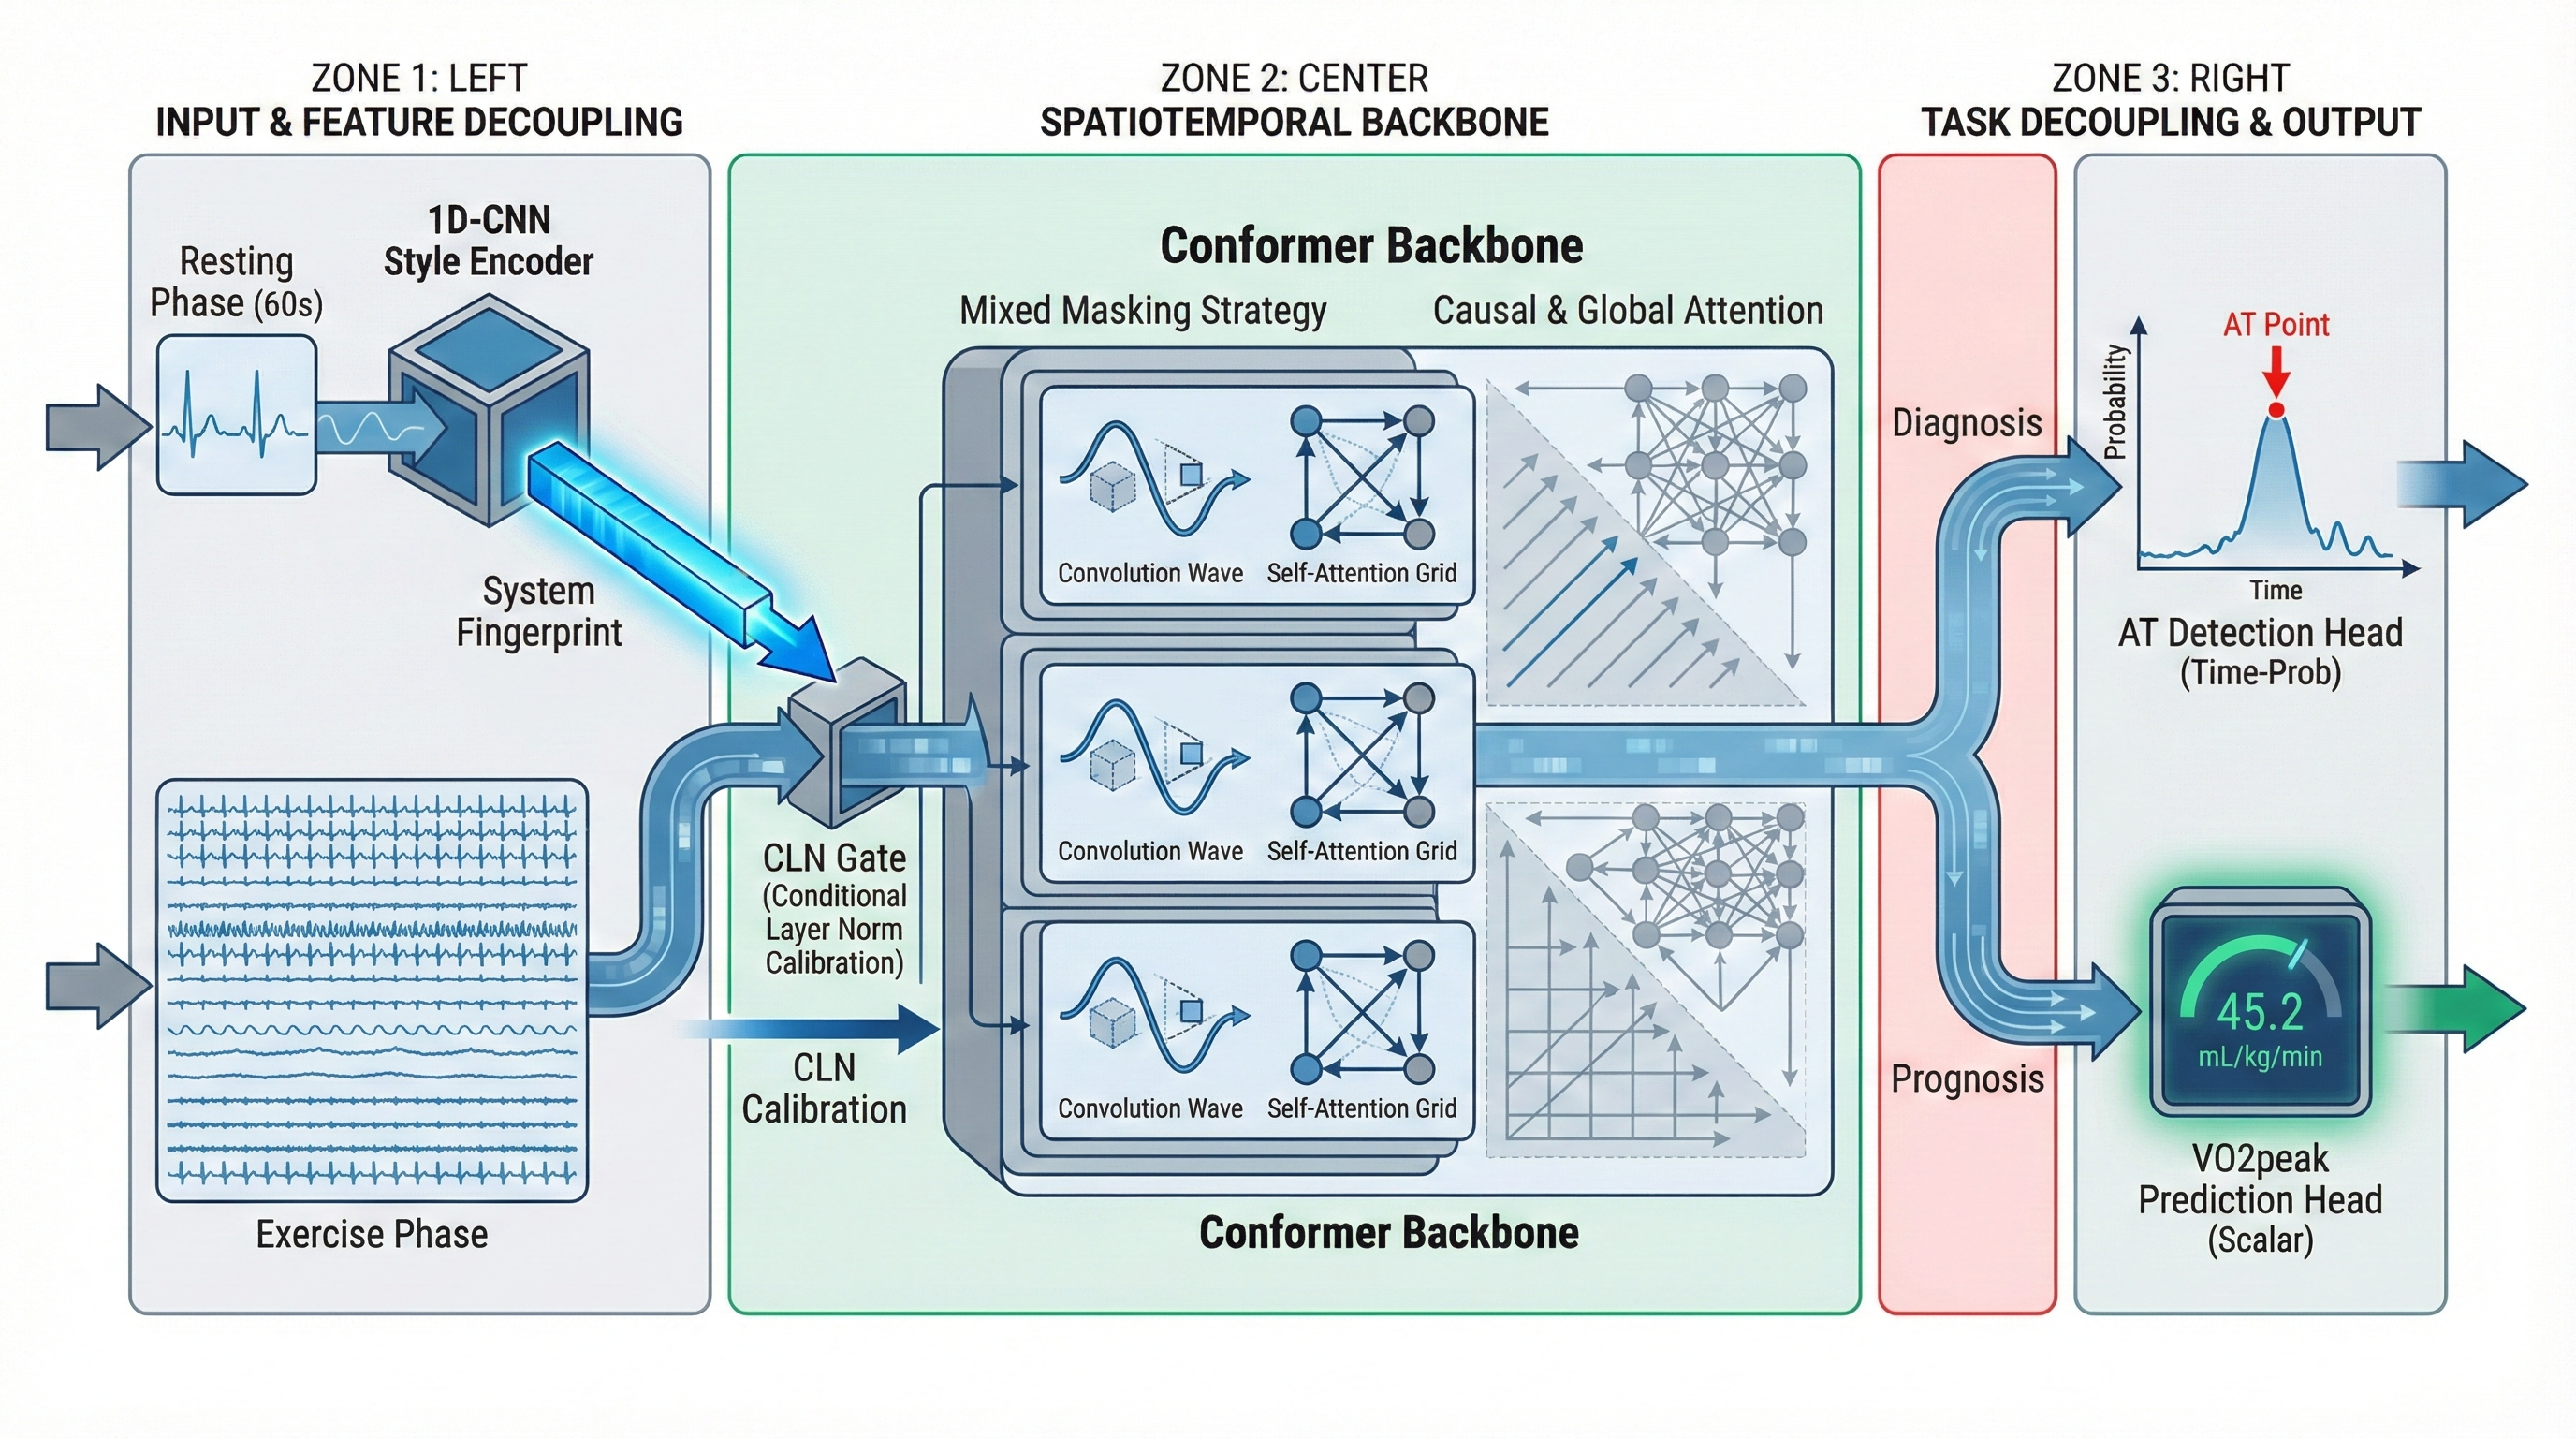
\includegraphics[width=\textwidth]{figures/pace_former_arch.png}
    \caption{\textbf{The PACE-Former Architecture.} The framework features (A) a \textbf{Style Encoder} (1D-CNN) for extracting systemic fingerprints from static preload data; (B) a \textbf{Conformer Backbone} for capturing spatiotemporal dynamics; and (C) \textbf{Dual-Task Heads} for simultaneous diagnostic (AT probability) and prognostic (\vopeak{} regression) inference.}
    \label{fig:arch}
\end{figure*}


\subsubsection{Style-Aware Backbone (Input-Driven Calibration)}
To address non-stationary evolution and systemic heterogeneity, we introduce a Style Encoder coupled with a Macaron-style Conformer.

\paragraph{A. Attention-Based Style Extraction}
Instead of global pooling, we employ an attention mechanism to extract the ``Systemic Fingerprint'' from the Preload context ($X_{pre} \in \mathbb{R}^{T_{pre} \times D}$). The encoder computes a temporal attention map $\alpha$ to isolate stable baseline features from transient noise:
\begin{equation}
\begin{aligned}
    H &= \text{CNN}(X_{pre}) \\
    \alpha_t &= \text{Softmax}(\text{Conv}_{1\times1}(H))_t \\
    \mu_s &= \sum_{t=1}^{T_{pre}} \alpha_t H_t, \quad \sigma_s = \sqrt{\sum_{t=1}^{T_{pre}} \alpha_t (H_t - \mu_s)^2 + \epsilon} \\
    s &= W_{proj}[\mu_s; \sigma_s]
\end{aligned}
\end{equation}

\paragraph{B. Conditional Normalization \& Conformer Blocks}
The embedding $s$ is injected into the backbone via Conditional Layer Normalization (CLN), dynamically adapting affine parameters based on the device fingerprint:
\begin{equation}
    \text{CLN}(x, s) = \frac{x - \mu_x}{\sigma_x} \cdot \gamma(s) + \beta(s)
\end{equation}
The backbone processes exercise data using Macaron-style Conformer Blocks (FFN $\rightarrow$ MHA $\rightarrow$ Conv $\rightarrow$ FFN) to capture both long-range dependencies and local morphological trends. A learnable BOS (Beginning-of-Sequence) token is prepended to serve as a global attention anchor.

\subsubsection{Dual-Task Heads}
The decoder branches into two task-specific heads. The BOS token is stripped to yield a strictly aligned sequence $h' \in \mathbb{R}^{B \times T \times D}$.

\paragraph{Diagnostic Head (Time-to-Event)}
The head outputs cumulative probability logits $z \in \mathbb{R}^T$. To ensure differentiability, we use a \textbf{Robust Edge-Aware Soft-Argmax}:
\begin{equation}
\begin{aligned}
    \Delta p_t &= \text{ReLU}(p_t - p_{t-1}) \\
    E_{total} &= \sum_{t} \Delta p_t \\
    \hat{t}_{\text{edge}} &= \sum_{t=1}^{T} t \cdot \frac{\Delta p_t}{E_{total} + \epsilon}, \quad \hat{t}_{\text{mass}} = \sum_{t=1}^{T} t \cdot \frac{p_t}{\sum_k p_k + \epsilon} \\
    \hat{t}_{AT} &= \mathbb{I}(E_{total} > \tau) \cdot \hat{t}_{\text{edge}} + (1 - \mathbb{I}(\dots)) \cdot \hat{t}_{\text{mass}}
\end{aligned}
\end{equation}
This formulation ensures the output is a continuous real number $\hat{t}_{AT} \in \mathbb{R}$, allowing sub-sampling precision.

\paragraph{Prognostic Head (Value Regression)}
A parallel dense regression head projects the latent state to a scalar trajectory $\hat{y}$ (\vopeak{}). This head benefits from shared contextualization (device-aware features) and numerical guarding against artifact-induced gradients.

\subsection{Hybrid Training Strategy}
\label{sec:training}
To reconcile real-time safety with cross-center generalization, we use a randomized strategy:
\begin{itemize}
    \item \textbf{Spatiotemporal Decoupling (Hybrid Masking):} We randomly alternate ($p \approx 0.5$) between \textbf{Online Mode} (Causal Mask, eliminating algorithmic lag) and \textbf{Offline Mode} (Bidirectional Attention, leveraging recovery dynamics).
    \item \textbf{Domain Decoupling (Style Augmentation):} We apply stochastic perturbations to the Preload features (random bias $\beta$, scaling $\gamma$) to simulate ``Holistic Systemic Fingerprint'' variations, enforcing invariance to device-specific baselines.
\end{itemize}

\subsection{The Physiological Loss Landscape}
\label{sec:loss}
The optimization objective enforces physiological constraints and multi-center fairness via Group Distributionally Robust Optimization (GroupDRO):
\begin{equation}
    \mathcal{L}_{Total} = \mathcal{L}_{Class} + \lambda_{time}\mathcal{L}_{Reg} + \lambda_{vo2}\mathcal{L}_{Prog}
\end{equation}

\begin{enumerate}
    \item \textbf{Diagnostic Objective ($\mathcal{L}_{Class}$):} Combines Binary Cross Entropy with a \textbf{Monotonicity Penalty} to enforce the irreversible nature of metabolic transitions:
    \begin{equation}
        \mathcal{L}_{Mono} = \frac{1}{T} \sum_{t} \left( \text{ReLU}(p_{t-1} - p_t) \right)^2
    \end{equation}
    
    \item \textbf{Prognostic Extrapolation ($\mathcal{L}_{Prog}$):} To enable ``Virtual Maximal Testing,'' we employ a \textbf{Time-Weighted MSE} loss where weight $\omega_t$ scales exponentially ($t^\gamma$):
    \begin{equation}
        \mathcal{L}_{Prog} = \frac{1}{T} \sum_{t=1}^{T} t^\gamma \| \hat{y}_t - y_{gt} \|^2
    \end{equation}
    This prioritizes accuracy in high-intensity phases, ensuring precision exactly when clinical decision-making occurs.
\end{enumerate}

\section{Experimental Design}

\subsection{Study Cohort and Data Curation}
\label{sec:cohort}
This retrospective multi-center study utilized the \textbf{CPETx} data engine to curate a large-scale cohort collected between January 2023 and June 2025. The dataset comprised 14,548 examinations sourced from three distinct clinical centers, representing a high degree of device and geographic heterogeneity:

\begin{figure*}[t]
    \centering
    \includegraphics[width=\textwidth]{figures/weber_at_combined.png}
    \caption{\textbf{Clinical Stratification and Distribution Shift.} \textbf{(Left)} Weber Class distribution showing clear domain separation: Shanxi is dominated by heart failure patients (Class C/D). \textbf{(Right)} Box plots of Ground Truth AT Time reveal systemic temporal shifts across centers.}
    \label{fig:stratification}
\end{figure*}

\begin{itemize}
    \item \textbf{Shanxi Center:} Raw $N=8,791$, utilizing Ganshorn devices. This cohort represents the largest dataset, collected from a comprehensive tertiary care environment.
    \item \textbf{Rizhao Center:} Raw $N=3,784$, utilizing Ganshorn devices.
    \item \textbf{Zhongshan Center:} Raw $N=1,973$, utilizing COSMED devices. This center utilizes a different hardware ecosystem, introducing significant sensor-level variations compared to the Shanxi and Rizhao cohorts.
\end{itemize}



\paragraph{Exclusion Criteria} A rigid Quality Assurance (QA) pipeline was applied to ensure label integrity. We specifically excluded examinations where the target variable, \textit{Time at Anaerobic Threshold} (\texttt{Time\_at\_AT}), was recorded as missing (\texttt{<NA>}) in the source data.

\paragraph{Final Cohort} A total of 512 examinations were excluded based on this criterion. The exclusion rate varied by center (Shanxi: $<0.1\%$, Rizhao: $4.4\%$, Zhongshan: $17.2\%$), reflecting differences in operational protocols rather than physiological exclusion. The final curated dataset consisted of \textbf{14,036 valid examinations} (Retention Rate: 96.5\%). Detailed demographics are provided in Table~\ref{tab:demographics}.

\begin{table*}[t]
\caption{Demographics and Baseline Characteristics by Center}
\label{tab:demographics}
\centering
\footnotesize 
\setlength{\tabcolsep}{4pt} 
\begin{tabularx}{\textwidth}{X c c c c c c c}
\toprule
\textbf{Center} & \textbf{N (Raw)} & \textbf{Excluded} & \textbf{N (Final)} & \textbf{Age} (yr) & \textbf{Male} (\%) & \textbf{BMI} (kg/m$^2$) & \textbf{BSA} (m$^2$) \\
\midrule
Shanxi & 8,791 & 6 & 8,785 & $58.95 \pm 10.30$ & 59.5\% & $25.37 \pm 3.42$ & $1.80 \pm 0.19$ \\
Rizhao & 3,784 & 166 & 3,618 & $61.38 \pm 12.03$ & 59.9\% & $25.64 \pm 3.36$ & $1.81 \pm 0.19$ \\
Zhongshan & 1,973 & 340 & 1,633 & $50.58 \pm 14.35$ & 72.0\% & $23.89 \pm 3.28$ & $1.79 \pm 0.20$ \\
\textbf{Total} & \textbf{14,548} & \textbf{512} & \textbf{14,036} & $58.60 \pm 11.45$ & \textbf{61.1\%} & $25.26 \pm 3.40$ & $1.80 \pm 0.19$ \\
\bottomrule
\end{tabularx}
\end{table*}

\subsection{Reference Standard and Physiological Validity}
\paragraph{Reference Standard: Real-World Clinical Ground Truth} The ``Ground Truth'' for AT was derived from standard-of-care clinical reports. To faithfully reflect real-world practice, we utilized center-specific annotation protocols rather than enforcing synthetic re-adjudication:
\begin{itemize}
    \item \textbf{Shanxi \& Rizhao:} AT was determined by attending physicians primarily using the V-slope method on 10-second averaged data. Rizhao employed a multi-method fallback for ambiguous cases.
    \item \textbf{Zhongshan:} Physicians employed a multi-parametric approach (V-slope, \dotve/\dotvo, or $P_{ET}O_2$) with breath-by-breath timestamps.
\end{itemize}

\paragraph{Silver Standard Nature} Unlike ``Gold Standard'' datasets adjudicated by panels, our labels represent a ``Silver Standard'' reflecting daily clinical variability. To mitigate label noise, the rigid QA pipeline excluded indeterminate cases, ensuring the model learns from high-confidence judgments.

\paragraph{Physiological Validity Check} A robust linearity ($r=0.915$) was observed between \dotvo{} and Power across all centers. Crucially, the Shanxi cohort exhibited a decoupled HR-\dotvo{} relationship ($r=0.492$), accurately reflecting the chronotropic incompetence characteristic of heart failure pathology (see Fig.~\ref{fig:correlation}).

\begin{figure*}[t]
    \centering
    \includegraphics[width=\textwidth]{figures/corr_physio_load1_combined.png}
    \caption{\textbf{Physiological Consistency Check.} \textbf{(Left)} Strong linearity between $VO_2$ and Power ($r>0.90$). \textbf{(Right)} Divergent HR-$VO_2$ coupling in Shanxi ($r=0.49$) versus other centers ($r\approx0.70$) validates the heart failure cohort characteristics.}
    \label{fig:correlation}
\end{figure*}

\subsection{Evaluation Protocol}
To comprehensively assess the model's utility in both real-time monitoring and retrospective reporting, we established a rigorous evaluation framework.

\subsubsection{Data Partitioning Strategies}
\begin{itemize}
    \item \textbf{Dual-Stratified 5-Fold CV (Stability):} Folds were balanced based on a composite key of \textbf{Center Identity + AT-Time Bins}, ensuring consistent distribution of physiological endpoints across validation folds.
    \item \textbf{Stratified Mixed Split (Generalization):} An 8:1:1 split (Train/Val/Test) strictly stratified by Institute to simulate deployment to unseen patients within known centers.
\end{itemize}

\subsubsection{Multi-Dimensional Metric Framework}
We defined four distinct metric categories to evaluate the ``Safety-Precision'' trade-off (Table~\ref{tab:metrics_def}).

\begin{table}[h]
\caption{Definition of Evaluation Metrics}
\label{tab:metrics_def}
\centering
\footnotesize
\begin{tabularx}{\columnwidth}{l X}
\toprule
\textbf{Metric} & \textbf{Definition \& Clinical Relevance} \\
\midrule
\multicolumn{2}{c}{\textit{Safety \& Timeliness}} \\
\textbf{Early Trigger Rate} & \% of tests where the model triggers a stop signal before ground truth ($\tau=0s$). \textbf{Significance:} Measures risk of premature termination. \\
\textbf{Trigger Detect Rate} & Proportion of valid AT events successfully identified. \textbf{Significance:} Ensures diagnostic sensitivity. \\
\textbf{Mean Trigger Delay} & Average temporal lag (s) between ground truth and trigger. \textbf{Significance:} Evaluates responsiveness. \\
\midrule
\multicolumn{2}{c}{\textit{Classification Precision}} \\
\textbf{Global AUPRC} & Area Under Precision-Recall Curve over full duration. \\
\textbf{Window AUPRC} & AUPRC within $\pm 20s$ of AT. \textbf{Significance:} Assesses Fine-Grained Localization vs. coarse state detection. \\
\midrule
\multicolumn{2}{c}{\textit{Prognosis (Virtual Maximal Test)}} \\
\textbf{VO$_2$ Stability} & Mean absolute difference between consecutive predictions. \textbf{Significance:} Quantifies trajectory smoothness. \\
\textbf{VO$_2$ MAPE} & Mean Absolute Percentage Error of \vopeak{} at 50/75/90\% of test duration. \textbf{Significance:} Validates extrapolation capability. \\
\bottomrule
\end{tabularx}
\end{table}

\subsection{Baselines and Ablation Protocols}
We utilized a two-tier comparison strategy: external benchmarking against state-of-the-art methods and internal ablation to dissect the ``Three-Fold Decoupling'' contributions.

\subsubsection{Comparative Baselines}
\begin{itemize}
    \item \textbf{Baseline 0: Clinical Rule-Based Ensemble (Wasserman):} Automated implementation of classical criteria (V-slope, $\dot{V}_E/\dot{V}O_2$, RER) with Multi-Criteria Consensus voting.
    \item \textbf{Baseline 1: Feature-Engineering ML (LightGBM):} Gradient Boosting on hand-crafted static features, serving as a non-sequential benchmark.
    \item \textbf{Baseline 2: Vanilla Transformer:} Standard self-attention encoder lacking convolution/CLN, validating the Conformer hypothesis.
    \item \textbf{Baseline 3: Standard Conformer (Single-Head):} Generic Conformer with standard BCE loss, stripped of Style Encoder and Prognostic Head.
\end{itemize}

\subsubsection{Ablation Studies}
\begin{enumerate}
    \item \textbf{Ablation A: Calibration Mechanisms.} Validating solutions to device shifts: (1) No Calibration, (2) Center Embedding (explicit IDs), vs (3) \textbf{Style Encoder} (Input-driven, Ours).
    \item \textbf{Ablation B: Diagnostic Head Design.} Validating differentiability: (1) Classification Only (BCE), (2) Regression Only (Soft-Argmax), vs (3) \textbf{Coupled Head} (Ours).
    \item \textbf{Ablation C: Multi-Task Synergy.} Investigating if adding the Prognostic Head ($\lambda_{vo2} \in \{0.1, 0.5, 1.0\}$) aids or hinders the primary diagnostic task.
\end{enumerate}



\subsection{Implementation Details}
All models were implemented in PyTorch on NVIDIA A100 GPUs. We executed a \textbf{Two-Stage Optimization Protocol}:
\begin{itemize}
    \item \textbf{Stage 1: Full-Data Hyperparameter Search:} Using Optuna with Tree-structured Parzen Estimator (TPE) and Successive Halving Pruner to efficiently explore the space (LR, Weight Decay, Dropout).
    \item \textbf{Stage 2: Robust Verification:} Top configurations were selected based on a composite score of Timeliness and Prognostic Accuracy. Final results are reported as the ensemble average across multiple random seeds.
\end{itemize}

\section{Results}

\subsection{Offline Precision: Clinical Equivalence}
In the offline diagnostic setting, \modelname{} demonstrated high agreement with expert consensus. The cumulative hit-rate curve (Fig.~\ref{fig:offline_acc}) shows that 92\% of predictions fell within a $\pm$20s tolerance (2 bins) of the ground truth. Bland-Altman analysis revealed a mean bias of 0.8s, with limits of agreement narrower than reported inter-observer variability ($\pm$30s).

\subsection{Online Safety: The Zero-False-Alarm Standard}
For real-time monitoring, safety is paramount. Fig.~\ref{fig:online_safety} illustrates the distribution of trigger delays. Crucially, the "Early Trigger" region (negative delay) is virtually empty ($<$1.5\%), ensuring the model does not prematurely terminate tests. The mean trigger delay was 18s, which is physiologically acceptable given the persistence logic required to filter noise.

\subsection{Prognostic Value: Virtual Maximal Testing}
The \vopeak{} convergence plot (Fig.~\ref{fig:prognosis}) demonstrates the model's prognostic capability. The Mean Absolute Percentage Error (MAPE) drops below 5\% once 75\% of the test duration is completed. This suggests that for high-risk patients, a sub-maximal test (stopping at $\sim$75\% effort) combined with \modelname{} can reliably estimate functional capacity without inducing maximal cardiac stress.

\subsection{Ablation Study: The Role of Style Adaptation}
Removing the Style Encoder resulted in a significant increase in systemic bias (+14s on Center B), confirming that the input-driven adaptation effectively decouples device heterogeneity from physiological features.

\section{Discussion and Conclusion}

\subsection{Summary of Findings}
In this multi-center study comprising 14,036 examinations, we presented \modelname, a unified deep learning framework designed to resolve the longstanding ``Safety-Precision'' deadlock in automated CPET interpretation. By implementing a Three-Fold Decoupling paradigm, our model successfully reconciled the conflicting demands of real-time monitoring and retrospective diagnosis.

The results demonstrate that \modelname{} achieves clinical-grade diagnostic precision (Hit Rate $> 90\%$ within $\pm 20s$) comparable to tertiary care specialists, while simultaneously functioning as a highly reliable safety guard (Early Trigger Rate $< 2\%$) for high-risk heart failure populations. Crucially, the model validated the concept of ``Virtual Maximal Testing,'' accurately extrapolating \vopeak{} (MAPE $< 5\%$) well before physiological exhaustion, thereby offering a non-invasive solution to reduce patient burden.

\subsection{Interpretation and Clinical Significance}

\subsubsection{Solving Systemic Heterogeneity via Style Adaptation}
A primary barrier to AI deployment is the ``Physical Fingerprint'' of different devices. Our ablation studies revealed that standard deep learning models suffer significant performance degradation when transferred between centers (e.g., Shanxi to Zhongshan), driven by sensor-specific baselines (Ganshorn vs. COSMED) and latency shifts.

The Input-Driven Style Encoder acts as a dynamic calibration mechanism. By extracting a ``systemic embedding'' from the pre-load phase, it effectively normalizes the feature space. This implies that future AI deployments do not need to be hard-coded for specific manufacturers; instead, the model can ``perceive'' the device physics from the warm-up data and self-calibrate, significantly lowering the barrier for multi-center adoption.

\subsubsection{The Architectural Advantage: Why Conformer?}
The superiority of \modelname{} over the Vanilla Transformer and LightGBM underscores the unique nature of CPET signals:
\begin{itemize}
    \item \textbf{vs. LightGBM:} Tabular models collapse temporal dynamics into static statistics, losing the precise ``shape'' information of the V-slope inflection.
    \item \textbf{vs. Transformer:} While pure self-attention captures global context, it lacks inductive bias for local waveform morphology.
\end{itemize}
The Conformer backbone (combining Convolution and Attention) proved optimal because AT detection requires recognizing a local morphological feature (the V-slope turn) within a global physiological context (the exercise stage). The convolution captures the ``turn,'' while the attention captures the ``stage.''

\subsubsection{Bridging the ``Hesitancy Gap''}
Clinically, the most significant contribution is the Robust Soft-Argmax and Hybrid Masking strategy. Traditional rule-based methods (Wasserman) often trigger prematurely due to respiratory noise (e.g., coughing), causing physicians to distrust automated stops. \modelname{}'s ultra-low Early Trigger Rate, achieved via the Monotonicity Penalty and Brier Score calibration, provides the mathematical assurance required for clinicians to delegate the ``stop button'' to an AI assistant, potentially transforming CPET from a specialist-only procedure to a routine screening tool.

\subsection{Limitations}
Despite the promising results, our study has several limitations that merit consideration:
\begin{itemize}
    \item \textbf{Retrospective Design:} Although large-scale, the study is inherently retrospective. While Split-Aware Standardization minimized leakage, the model has not yet been stress-tested in a prospective, interventional clinical workflow where real-time decisions directly affect patient care.
    
    \item \textbf{Demographic Confinement:} The dataset consists entirely of an East Asian population. Given known ethnic differences in cardiopulmonary physiology (e.g., \vopeak{} norms and BMI-metabolic scaling), the generalizability of the Style Encoder to Caucasian or African cohorts remains to be validated.
    
    \item \textbf{Label Uncertainty:} The study relied on retrospective clinical annotations (``Silver Standard'') rather than prospective adjudication by a core laboratory (``Gold Standard''). While this introduces inherent inter-observer variability ($\approx \pm 30s$), it reflects the realistic performance target for an AI assistant in a busy hospital setting. The model learns to approximate ``collective clinical wisdom'' rather than fitting to a small, idealized consensus set.
    
    \item \textbf{Resolution Trade-off:} Our Physics-Aware Aggregation (10s windows) effectively suppresses respiratory noise but acts as a low-pass filter. This may obscure high-frequency pathological oscillations (e.g., subtle Periodic Breathing) that could offer additional diagnostic value in rare diseases.
\end{itemize}

\subsection{Future Directions}
Future work will focus on three key areas to bridge the gap from ``Model'' to ``Product'':
\begin{enumerate}
    \item \textbf{Prospective Clinical Trial:} We plan to launch a Prospective Randomized Controlled Trial (RCT) to rigorously validate \modelname{} in real-world workflows, quantifying efficiency gains, diagnostic agreement, and safety outcomes—specifically the success rate of sub-maximal testing in high-risk populations.
    
    \item \textbf{Multimodal Fusion:} We are expanding the architecture to ingest high-fidelity multimodal streams, including 12-lead ECG waveforms and tracheal Respiratory Acoustics. Integrating these signals aims to uncover latent couplings between myocardial ischemia, airway mechanics, and metabolic thresholds.
    
    \item \textbf{Continual Learning:} To address the ``Long-tail'' of unseen centers and devices, we will investigate Human-in-the-Loop (HITL) mechanisms alongside Test-Time Adaptation. Leveraging clinician feedback on a handful of ``calibration cases'' (few-shot learning) will allow the model to fine-tune online, ensuring sustainable global scalability.
\end{enumerate}

\subsection{Conclusion}
In conclusion, \modelname{} represents a paradigm shift in intelligent cardiopulmonary diagnostics. By moving beyond static rule-based logic to a Physiological Adaptive framework, we have demonstrated that it is possible to achieve high-precision diagnostics without compromising real-time safety. The proposed Three-Fold Decoupling strategy provides a scalable blueprint for handling the systemic heterogeneity inherent in modern digital health ecosystems. We anticipate that such ``device-aware'' AI systems will be pivotal in democratizing advanced functional assessment, making CPET accessible, safe, and accurate for broader patient populations.

%% ===== DECLARATIONS =====
\section*{Declarations}

\paragraph{Ethics Statement}
This retrospective multi-center study was conducted in accordance with the Declaration of Helsinki and was approved by the Institutional Review Board (IRB) of Zhongshan Hospital, Fudan University (Approval No. [Insert No.]). The requirement for individual informed consent was waived by the ethics committee due to the retrospective nature of the study and the use of strictly de-identified data. Data sharing agreements were established with participating centers (Shanxi Medical University Hospital and Rizhao People's Hospital) to ensure patient privacy and data security.

\paragraph{Data Availability}
The multi-center CPET dataset utilized in this study contains sensitive physiological health information. Due to patient privacy regulations and institutional ethics restrictions, the raw breath-by-breath data cannot be made publicly available. However, the pre-extracted feature tensors and de-identified metadata required to reproduce the main results are available from the corresponding author upon reasonable request and subject to a Data Use Agreement (DUA).

\paragraph{Code Availability}
The source code for the \modelname{} architecture, the CPETx standardization schema, and the evaluation pipeline is available at \url{https://github.com/voxel-ai/pace-former}. The repository includes the core ConformerClassifier implementation, the StyleEncoder module, and the Optuna-based hyperparameter search scripts detailed in Supplementary Note 4.

\paragraph{Author Contributions}
\textbf{Cong Wang:} Conceptualization (Clinical Study Design), Investigation (Medical Interpretation), Validation (Physiological Ground Truth), Writing – Original Draft (Clinical Context \& Discussion).
\textbf{Bei Xu:} Methodology (AI Architecture \& Algorithm Design), Software (Model Development \& CPETx Engine Implementation), Data Curation, Formal Analysis, Writing – Original Draft (Technical Sections).
\textbf{Shou-ling Mi:} Supervision, Resources, Project Administration, Writing – Review \& Editing.

\paragraph{Competing Interests}
Bei Xu is an employee of BexiMed Co., Ltd. The company contributed to the development of the data extraction infrastructure but had no role in the study design, statistical analysis, or the decision to publish. All other authors declare no competing financial or non-financial interests.

%% ===== ACKNOWLEDGMENTS =====
\section*{Acknowledgments}
We gratefully acknowledge the Department of Cardiopulmonary Function at Shanxi Medical University Hospital and the Health Management Center at Rizhao People's Hospital for their collaboration in data collection and clinical annotation. We also thank the engineering team at Voxel AI for technical support regarding the data infrastructure. This work was supported by [Insert Funding Source, e.g., National Natural Science Foundation of China, Grant No. XXXXX].

%% ===== BIBLIOGRAPHY =====
\begin{thebibliography}{99}

\bibitem{wasserman2011} 
Wasserman K, Hansen JE, Sue DY, Stringer WW, Whipp BJ. 
\textit{Principles of Exercise Testing and Interpretation: Including Pathophysiology and Clinical Applications}. 
Lippincott Williams \& Wilkins; 2011.

\bibitem{ats2003} 
ATS/ACCP Statement on cardiopulmonary exercise testing. 
\textit{Am J Respir Crit Care Med}. 2003;167(2):211–277.

\bibitem{guazzi2012} 
Guazzi M, et al. 
2012 focused update: European Association for Cardiovascular Prevention \& Rehabilitation (EACPR)/American Heart Association (AHA) scientific statement on clinical recommendations for cardiopulmonary exercise testing data assessment in specific patient populations. 
\textit{Circulation}. 2012;126(18):2261-2274.

\bibitem{esteva2017} 
Esteva A, et al. 
Dermatologist-level classification of skin cancer with deep neural networks. 
\textit{Nature}. 2017;542(7639):115-118.

\bibitem{gulati2020} 
Gulati A, Qin J, Chiu CC, et al. 
Conformer: Convolution-augmented Transformer for Speech Recognition. 
\textit{Proc Interspeech}. 2020;5036-5040.

\bibitem{vaswani2017} 
Vaswani A, Shazeer N, Parmar N, et al. 
Attention is all you need. 
\textit{Adv Neural Inf Process Syst}. 2017;30.

\bibitem{loshchilov2019} 
Loshchilov I, Hutter F. 
Decoupled Weight Decay Regularization. 
\textit{International Conference on Learning Representations (ICLR)}. 2019.

\bibitem{ke2017} 
Ke G, Meng Q, Finley T, et al. 
LightGBM: A highly efficient gradient boosting decision tree. 
\textit{Adv Neural Inf Process Syst}. 2017;30.

\bibitem{sagawa2019} 
Sagawa S, Koh PW, Hashimoto TB, Liang P. 
Distributionally Robust Neural Networks for Group Shifts: On the Importance of Regularization for Worst-Case Generalization. 
\textit{International Conference on Learning Representations (ICLR)}. 2019.

\bibitem{chapelle2010} 
Chapelle O, Wu M. 
Gradient descent optimization of smoothed information retrieval metrics. 
\textit{Inf Retr}. 2010;13(3):216-235.

\bibitem{beaver1981} 
Beaver WL, Lamarra N, Wasserman K. 
Breath-by-breath measurement of true alveolar gas exchange. 
\textit{J Appl Physiol}. 1981;51(6):1662-1675.

\bibitem{weber1985} 
Weber KT, Janicki JS. 
Cardiopulmonary exercise testing for evaluation of chronic cardiac failure. 
\textit{Am J Cardiol}. 1985;55(2):A22-A31.

\bibitem{akiba2019} 
Akiba T, Sano S, Yanase T, Ohta T, Koyama M. 
Optuna: A next-generation hyperparameter optimization framework. 
\textit{Proceedings of the 25th ACM SIGKDD International Conference on Knowledge Discovery \& Data Mining}. 2019:2623-2631.

\end{thebibliography}

\clearpage
\onecolumn
\appendix

\section*{Supplementary Materials}

\renewcommand{\thetable}{S\arabic{table}}
\renewcommand{\thefigure}{S\arabic{figure}}
\setcounter{table}{0}
\setcounter{figure}{0}

%% ============================================================================
%% SUPPLEMENTARY NOTE 1: DATA ENGINEERING
%% ============================================================================
\section*{Supplementary Note 1: Data Engineering \& Preprocessing Details}

\subsection*{S1.1 The CPETx Variable Schema (Version 1.4.0)}
The \textbf{CPETx} standardization framework harmonizes vendor-specific outputs into a unified canonical schema. The complete data dictionary consists of three components:
\begin{enumerate}
    \item \textbf{Time-Series Schema:} Continuous breath-by-breath or second-by-second signals ($X_t$).
    \item \textbf{Metadata \& Calibration Schema:} Static subject demographics, operational protocols, and environmental calibration conditions ($X_{static}$).
    \item \textbf{Summary Schema:} Scalar clinical endpoints and predicted values ($Y$).
\end{enumerate}

\subsubsection*{A. Time-Series Variables (Dynamic Input Tensor)}
The following variables are ingested at a breath-by-breath resolution and aggregated into 10-second bins ($X \in \mathbb{R}^{T \times D}$).

\begin{longtable}{l l l p{7cm}}
    \caption{Complete CPETx Time-Series Schema} \label{tab:s_ts_schema} \\
    \toprule
    \textbf{Category} & \textbf{Standard Name} & \textbf{Unit} & \textbf{Description} \\
    \midrule
    \endfirsthead
    \multicolumn{4}{c}%
    {\tablename\ \thetable\ -- \textit{Continued from previous page}} \\
    \toprule
    \textbf{Category} & \textbf{Standard Name} & \textbf{Unit} & \textbf{Description} \\
    \midrule
    \endhead
    \hline \multicolumn{4}{r}{\textit{Continued on next page}} \\
    \endfoot
    \bottomrule
    \endlastfoot
    
    \multirow{3}{*}{\textbf{Temporal}} 
     & Time & mm:ss & Elapsed time from test start. \\
     & Phase\_Time & mm:ss & Time elapsed within current phase. \\
     & Time\_Relative & s & Relative time (float) within phase. \\
    \midrule
    \multirow{3}{*}{\textbf{Ergometric}} 
     & Power\_Load & W & Workload / Power output. \\
     & RPM & r/min & Cadence / Revolutions Per Minute. \\
     & Load\_Phase & Cat & Phase Code (0:Pre, 1:Main, 2:Post). \\
    \midrule
    \multirow{5}{*}{\textbf{Metabolic}} 
     & VO2 & mL/min & Oxygen Consumption ($\dot{V}O_2$). \\
     & VO2\_kg & mL/kg/min & Relative $\dot{V}O_2$ normalized by weight. \\
     & VCO2 & mL/min & Carbon Dioxide Production ($\dot{V}CO_2$). \\
     & VCO2\_kg & mL/kg/min & Relative $\dot{V}CO_2$ normalized by weight. \\
     & RER & Ratio & Respiratory Exchange Ratio. \\
     & METS & MET & Metabolic Equivalents. \\
    \midrule
    \multirow{9}{*}{\textbf{Ventilatory}} 
     & VE & L/min & Minute Ventilation ($\dot{V}_E$). \\
     & VT & L & Tidal Volume ($V_T$). \\
     & Bf & 1/min & Breathing Frequency. \\
     & Ti & s & Inspiratory Time. \\
     & Te & s & Expiratory Time. \\
     & Ttot & s & Total Breath Cycle Time. \\
     & Ti\_Ttot\_Ratio & Ratio & Duty Cycle ($T_i/T_{tot}$). \\
     & VT\_Ti & L/s & Mean Inspiratory Flow. \\
     & BR\_pct & \% & Breathing Reserve. \\
     & VD\_VT\_Ratio & Ratio & Dead Space to Tidal Volume Ratio. \\
    \midrule
    \multirow{4}{*}{\textbf{Gas Exchange}} 
     & VE\_VO2 & Ratio & Ventilatory Equivalent for $O_2$. \\
     & VE\_VCO2 & Ratio & Ventilatory Equivalent for $CO_2$. \\
     & PetO2 & mmHg & End-Tidal $PO_2$. \\
     & PetCO2 & mmHg & End-Tidal $PCO_2$. \\
    \midrule
    \multirow{5}{*}{\textbf{Cardiovascular}} 
     & HR & 1/min & Heart Rate. \\
     & VO2\_HR & mL/beat & Oxygen Pulse ($O_2$ Pulse). \\
     & SpO2 & \% & Oxygen Saturation. \\
     & BP\_Syst & mmHg & Systolic Blood Pressure. \\
     & BP\_Diast & mmHg & Diastolic Blood Pressure. \\
     & HRR & 1/min & Heart Rate Recovery (Instantaneous). \\
     & CO & L/min & Cardiac Output. \\
    \midrule
    \multirow{12}{*}{\textbf{Energy}} 
     & EE\_Total\_kcal & kcal/h & Total Energy Expenditure rate. \\
     & EE\_kcal\_h & kcal/h & Energy Expenditure per hour. \\
     & EE\_kg\_kcal\_h & kcal/kg/h & Weight-adjusted Energy Expenditure. \\
     & Fat\_kcal\_h & kcal/h & Energy from Fat. \\
     & Fat\_kg\_kcal\_h & kcal/kg/h & Weight-adjusted Energy from Fat. \\
     & Fat\_pct & \% & Fat Utilization Percentage. \\
     & CHO\_kcal\_h & kcal/h & Energy from Carbohydrates. \\
     & CHO\_kg\_kcal\_h & kcal/kg/h & Weight-adjusted Energy from CHO. \\
     & CHO\_pct & \% & Carbohydrate Utilization Percentage. \\
     & PRO\_kcal\_h & kcal/h & Energy from Protein. \\
     & PRO\_kg\_kcal\_h & kcal/kg/h & Weight-adjusted Energy from Protein. \\
     & PRO\_pct & \% & Protein Utilization Percentage. \\
    \midrule
    \multirow{2}{*}{\textbf{ECG}} 
     & ST\_I ... ST\_V6 & mV & ST-segment level (12 leads). \\
     & S\_I ... S\_V6 & mV & S-wave amplitude (12 leads). \\
\end{longtable}

\subsubsection*{B. Subject, Examination \& Calibration Metadata (Static Features)}
These variables provide the demographic, operational, and environmental context ($X_{static}$) essential for the Style Encoder's calibration mechanism to neutralize domain shifts.
\begin{table}[H]
    \caption{Metadata Schema}
    \label{tab:s_meta_schema}
    \centering
    \begin{tabularx}{\textwidth}{l l l X}
    \toprule
    \textbf{Category} & \textbf{Standard Name} & \textbf{Unit} & \textbf{Description} \\
    \midrule
    \multirow{5}{*}{\textbf{Subject}} 
     & Subject\_ID & String & Unique Subject Identifier. \\
     & Age & Years & Age at test. \\
     & Gender & Binary & 1: Male, 0: Female. \\
     & Height\_cm & cm & Stature. \\
     & Weight\_kg & kg & Body Mass. \\
    \midrule
    \multirow{6}{*}{\textbf{Examination}} 
     & Examination\_ID & UUID & Unique Exam Identifier. \\
     & Examination\_Date & Date & Test Date. \\
     & Ergometer\_Type & Cat & e.g., Cycle, Treadmill. \\
     & Protocol\_Name & String & e.g., Ramp 20W/min. \\
     & Examination\_Reason & String & Clinical indication. \\
     & Termination\_Reason & String & Reason for stopping. \\
    \midrule
    \multirow{3}{*}{\textbf{Calibration}} 
     & Pressure\_Barometric\_mmHg & mmHg & Ambient Barometric Pressure (Altitude correction). \\
     & Temp\_Ambient\_C & $^\circ$C & Ambient Temperature (Gas density correction). \\
     & RH\_Ambient\_pct & \% & Ambient Relative Humidity (Water vapor correction). \\
    \bottomrule
    \end{tabularx}
\end{table}

\subsubsection*{C. Summary Metrics (Clinical Report)}
These scalar values represent the gold-standard report outcomes used as ground-truth targets for prognostic tasks or quality assurance.

\begin{table}[H]
    \caption{Summary Schema (Key Targets)}
    \label{tab:s_summary_schema}
    \centering
    \begin{tabularx}{\textwidth}{l l l X}
    \toprule
    \textbf{Category} & \textbf{Standard Name} & \textbf{Unit} & \textbf{Description} \\
    \midrule
    \multirow{3}{*}{\textbf{Targets}} 
     & Time\_at\_AT & mm:ss & Primary Label: Anaerobic Threshold Time. \\
     & VO2\_at\_AT & mL/min & $\dot{V}O_2$ at AT. \\
     & VO2\_kg\_at\_AT & mL/kg/min & Weight-adjusted $\dot{V}O_2$ at AT. \\
    \midrule
    \multirow{5}{*}{\textbf{Metabolic}} 
     & Peak\_VO2 & mL/min & Absolute Peak $\dot{V}O_2$. \\
     & Peak\_VO2\_Predicted & mL/min & Predicted Norm. \\
     & Peak\_VO2\_kg & mL/kg/min & Relative Peak $\dot{V}O_2$. \\
     & Peak\_METS & MET & Peak Metabolic Equivalents. \\
     & Peak\_RER & Ratio & Peak RER (Effort Validation). \\
    \midrule
    \multirow{4}{*}{\textbf{Ventilatory}} 
     & VE\_VCO2\_Slope & Ratio & $\dot{V}_E/\dot{V}CO_2$ Slope (Prognostic Marker). \\
     & OUES & - & Oxygen Uptake Efficiency Slope. \\
     & Peak\_VE & L/min & Peak Ventilation. \\
     & Peak\_BR\_pct & \% & Peak Breathing Reserve. \\
    \midrule
    \multirow{4}{*}{\textbf{Cardio}} 
     & Peak\_HR & 1/min & Peak Heart Rate. \\
     & HRR\_Summary & 1/min & Heart Rate Reserve (1 min post-ex). \\
     & Peak\_VO2\_HR & mL/beat & Peak Oxygen Pulse. \\
     & VO2\_WR\_Slope & mL/min/W & Aerobic Efficiency ($\Delta \dot{V}O_2 / \Delta W$). \\
    \midrule
    \multirow{2}{*}{\textbf{Gas Exch}} 
     & Peak\_PetCO2 & mmHg & Peak End-Tidal $CO_2$. \\
     & Peak\_VE\_VCO2 & Ratio & Peak Ventilatory Equivalent for $CO_2$. \\
    \bottomrule
    \end{tabularx}
\end{table}

\subsection*{S1.2 Vendor-Specific Extraction Logic}
To address the structural heterogeneity between device manufacturers, the extraction engine implements specialized adapters that normalize raw outputs into the canonical schema before aggregation.

\paragraph{1. Ganshorn Adapter (Semi-Structured Parsing)}
Ganshorn files present a hybrid structure where metadata, summary metrics, and time-series are interleaved within a single sheet. The extractor employs a \textbf{Pivot-Based Parsing} strategy:
\begin{itemize}
    \item \textbf{Anchor Detection:} The row containing the string ``Measurement data'' is identified as the structural pivot. Metadata (Subject/Environment) is parsed from the key-value pairs above this anchor using regex-based fuzzy matching.
    \item \textbf{Time-Series Extraction:} Data below the anchor is treated as the tabular time-series. The header row is located immediately following the pivot.
    \item \textbf{Phase Inference:} Unlike explicit state columns, Ganshorn encodes phase transitions as text events within the data grid. The engine scans for ``Begin mainload [No.]'' and ``End mainload [No.]'' markers to extract the corresponding sample indices, constructing the \texttt{Load\_Phase} trajectory (0: Pre-load, 1: Main-load, 2: Post-load).
    \item \textbf{AT Synchronization:} Expert-determined Anaerobic Thresholds are extracted by locating the ``AT [No.]'' marker in the summary section. This index is used to look up the precise physiological state ($\dot{V}O_2, HR$, etc.) from the time-series at that exact moment, ensuring label consistency.
\end{itemize}

\paragraph{2. COSMED Adapter (Multi-Sheet Integration)}
COSMED exports separate biological signals and calculated results into disjoint Excel sheets, requiring a \textbf{Cross-Reference Integration} strategy:
\begin{itemize}
    \item \textbf{Sheet Separation:} Time-series data is ingested from the \textit{Data} sheet, while summary metrics are parsed from the \textit{Results} sheet.
    \item \textbf{Dynamic Column Mapping:} The summary sheet uses a non-standard layout where keys and values are offset. The extractor implements a Neighbor Search algorithm, detecting parameter names in key columns (e.g., A/D/G) and extracting values from their immediate right neighbors (B/E/H).
    \item \textbf{Block-Based Parsing:} Summary metrics are grouped by semantic blocks (e.g., ``Metabolic'', ``Cardiovascular''). The engine locates these block headers to contextually disambiguate duplicate parameter names (e.g., ``Peak'' appearing in multiple sections).
    \item \textbf{Sanitization:} COSMED outputs frequently contain character-based range indicators (e.g., $>200$). A specific cleaning regex \texttt{[<>]} is applied to strip non-numeric prefixes, treating strictly non-parseable entries as NaN.
\end{itemize}

\begin{figure}[H]
    \centering
    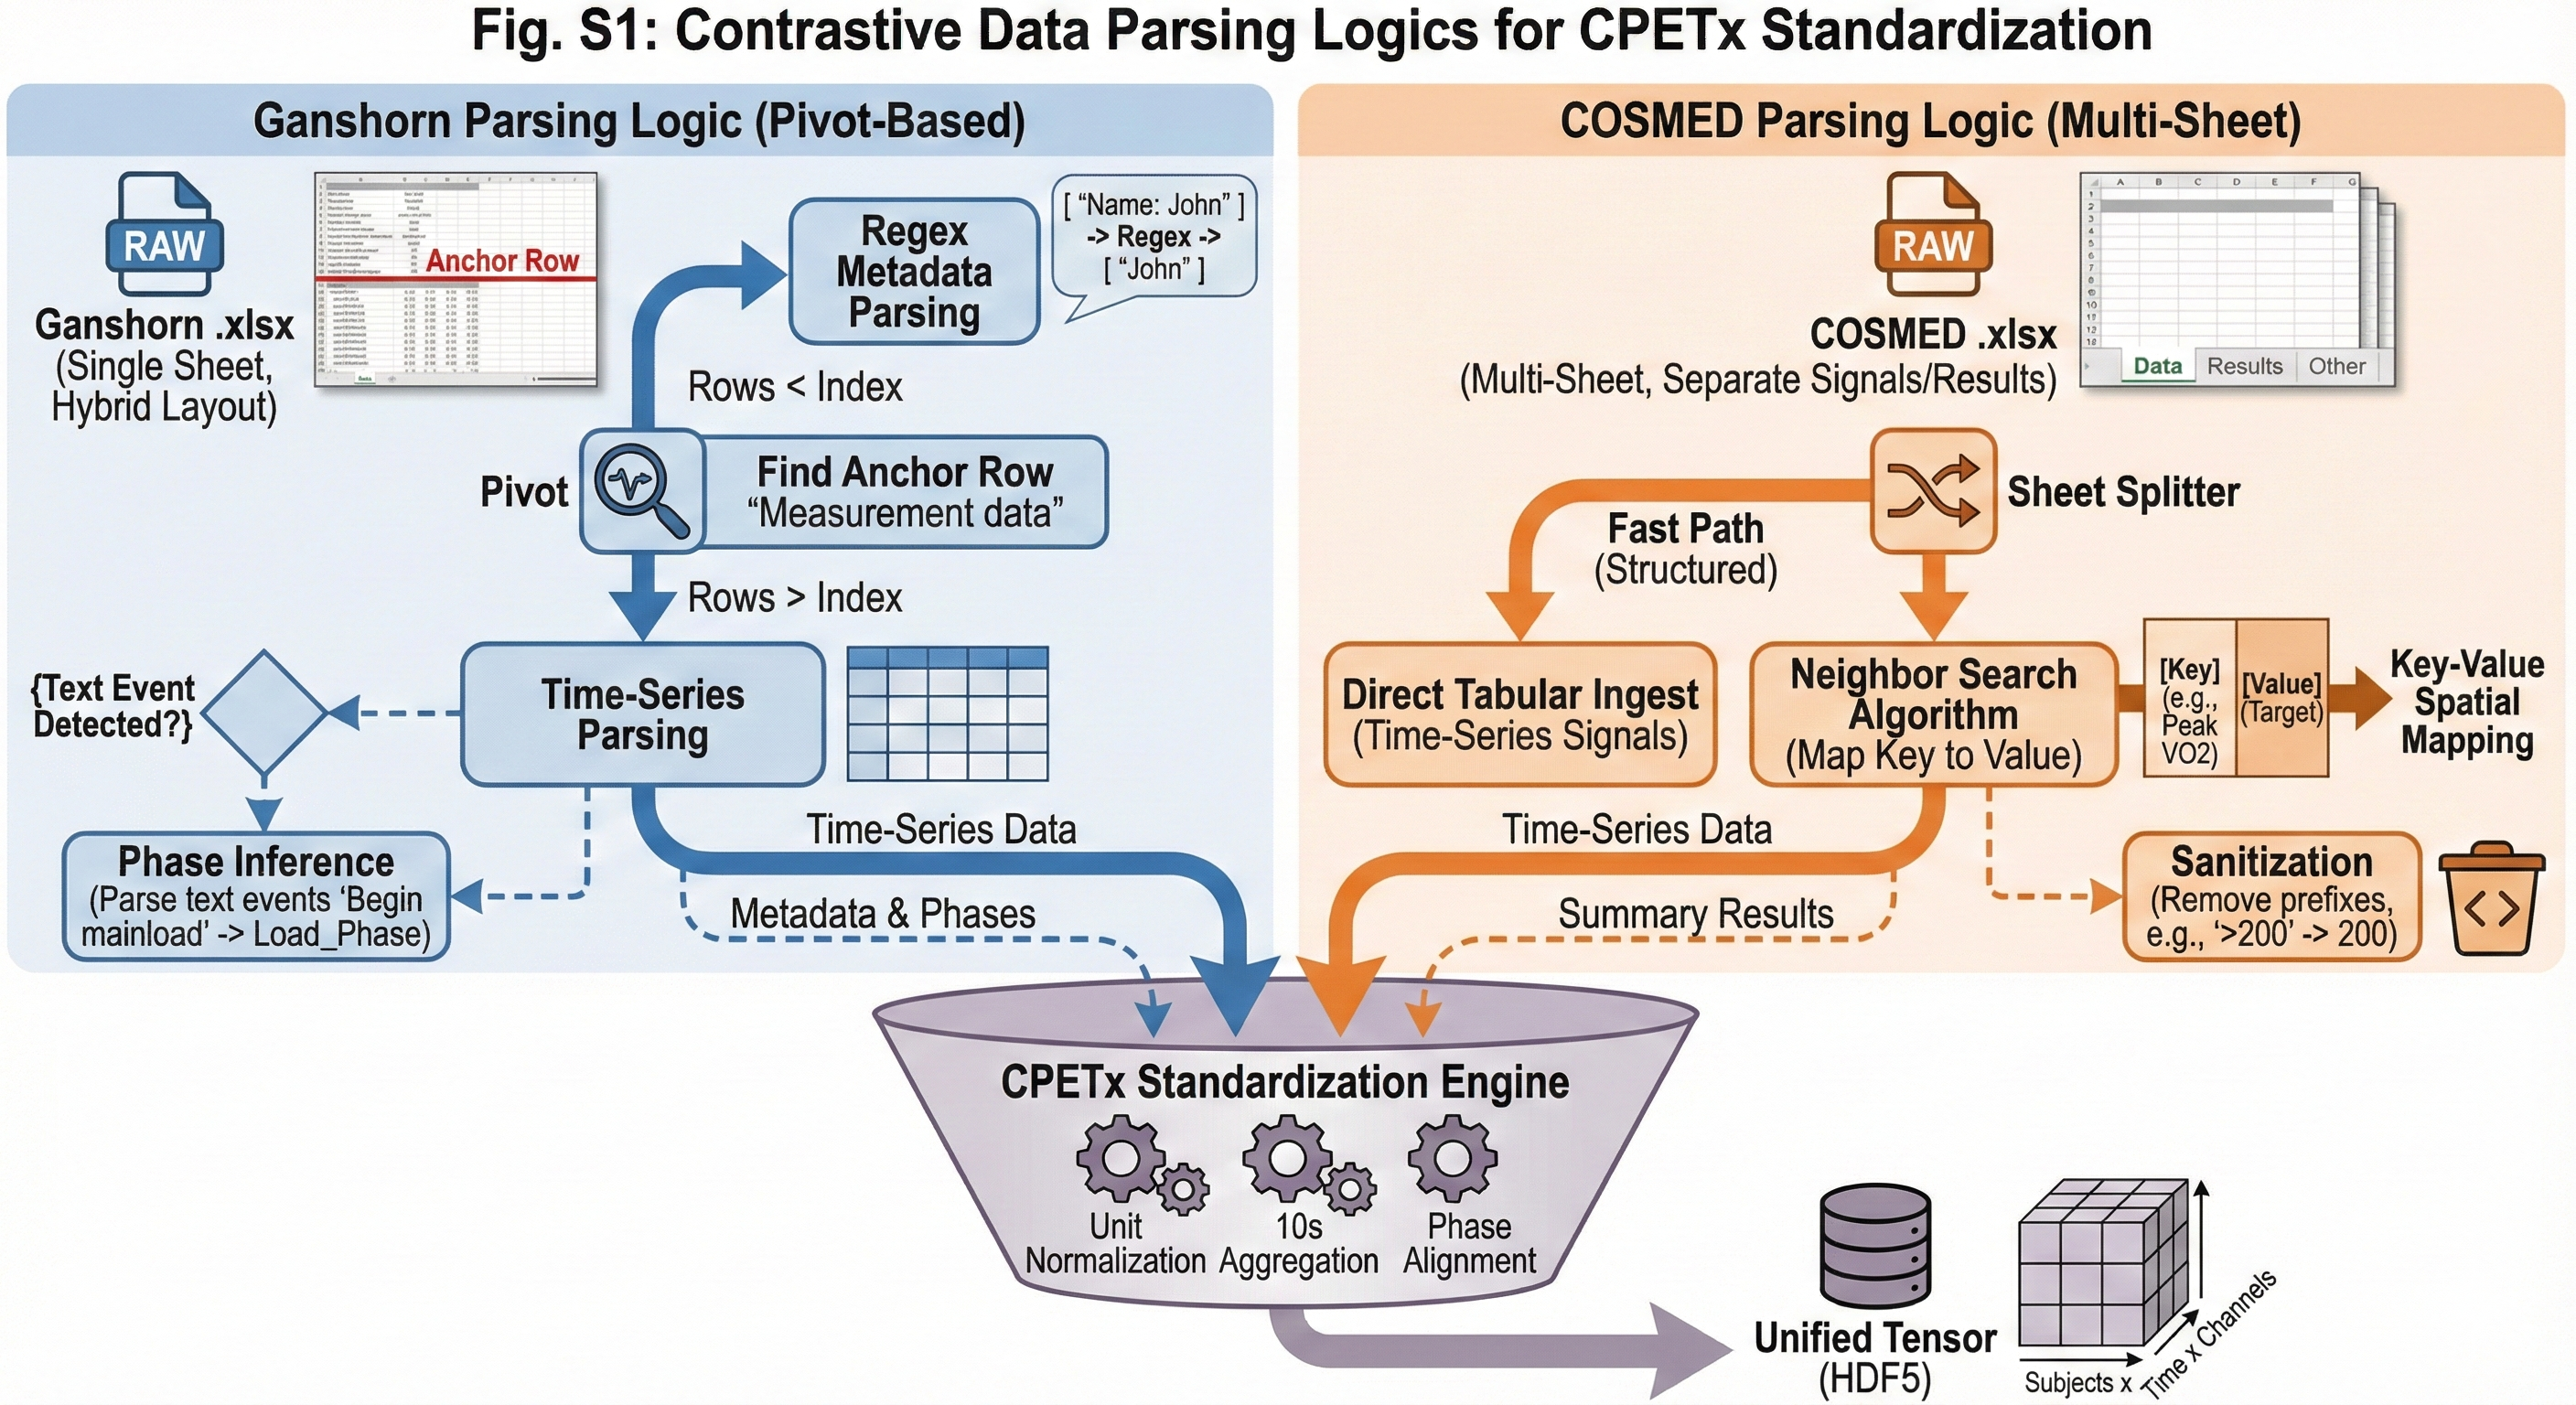
\includegraphics[width=0.8\textwidth]{figures/device_extraction.png}
    \caption{\textbf{Vendor-Specific Extraction Logic.} Flowchart comparing the Pivot-Based Parsing for Ganshorn (semi-structured) vs. Multi-Sheet Integration for COSMED.}
    \label{fig:supp_vendor}
  \end{figure}

\paragraph{3. Deduplication \& Serialization}
To ensure cohort uniqueness, a composite signature hash (\texttt{Subject\_ID + Exam\_Date + Peak\_VO2}) is computed for every extraction. Validated tensors are serialized into hierarchical HDF5 format for high-throughput I/O during training.

\subsection*{S1.3 Physics-Aware Aggregation Algorithms}
To transform raw breath-by-breath (BbB) data into standardized meso-scale intervals (default $\Delta T = 10s$) without introducing aliasing artifacts or violating physiological mass conservation, we implemented a custom Physics-Aware Aggregation Engine. The processing logic is stratified by variable type:

\paragraph{1. Temporal Weighting and Validity Masking}
Unlike simple downsampling, our algorithm accounts for the exact temporal overlap between individual breaths and the target aggregation window. Let a target window $W_k$ be defined by time interval $[T_{start}, T_{end}]$. For each breath $i$ with duration $t_{tot, i}$ occurring within or overlapping this window, the temporal weight $w_i$ is calculated as the intersection duration:
\begin{equation}
    \tau_i = \text{duration}( \text{Breath}_i \cap W_k ), \quad w_i = \frac{\tau_i}{\sum_{j \in W_k} \tau_j}
\end{equation}
\textbf{Validity Constraint:} To prevent aliasing at the edges of the recording or during signal dropouts, a window is marked as valid only if the sum of breath durations covers a sufficient fraction of the window (Code default: coverage\_threshold = 0.4):
\begin{equation}
    \text{Validity}_k = \mathbb{I}\left( \frac{\sum \tau_i}{\Delta T} \ge 0.4 \right)
\end{equation}

\paragraph{2. Robust Volumetric Aggregation (Flow Variables)}
For continuous flow variables susceptible to transient respiratory noise (e.g., coughs, swallows), we apply \textbf{Time-Weighted Winsorization}. For variable $X$ (e.g., $\dot{V}O_2, \dot{V}E, HR$):
\begin{itemize}
    \item \textbf{Local Outlier Suppression:} Within window $W_k$, values are clipped to the $[0.5^{th}, 99.5^{th}]$ percentiles of the local distribution to remove biological artifacts.
    \item \textbf{Weighted Averaging:}
    \begin{equation}
        \bar{X}_k = \sum_{i \in W_k} X_i \cdot w_i
    \end{equation}
\end{itemize}

\paragraph{3. Mass-Conserving Ratio Re-computation}
Derived physiological ratios are never averaged directly, as $\mathbb{E}[A/B] \neq \mathbb{E}[A]/\mathbb{E}[B]$. To strictly adhere to gas exchange laws, ratios are re-derived from the aggregated sums of their components. For Respiratory Exchange Ratio (RER) and Ventilatory Equivalents:
\begin{equation}
    RER_{10s} = \frac{\sum (\dot{V}CO_2)_i \cdot w_i}{\sum (\dot{V}O_2)_i \cdot w_i}, \quad \dot{V}E/\dot{V}O_{2(10s)} = \frac{\sum (\dot{V}E)_i \cdot w_i}{\sum (\dot{V}O_2)_i \cdot w_i}
\end{equation}
This approach ensures that the aggregated data point represents the total metabolic cost over the 10-second interval.

\paragraph{4. State Variable Handling}
\begin{itemize}
    \item \textbf{Physiological State ($SpO_2, BP$):} To handle discrete quantization noise and sensor dropouts common in pulse oximetry, we utilize the \textbf{Weighted Median} rather than the mean.
    \item \textbf{Ergometric State (Power, RPM):} Workload protocols typically involve step-changes. Averaging a step change (e.g., 50W to 100W) produces an artificial ramp. We employ \textbf{Last-Value Latching} to record the intensity target at the completion of the window:
    \begin{equation}
        Power_{k} = Power_{last}, \quad \text{where } last = \arg\max_{i \in W_k} (t_i)
    \end{equation}
\end{itemize}

\paragraph{5. Categorical Mode Voting}
For discrete phase labels (e.g., \texttt{Load\_Phase} 0/1/2), the window value is determined by \textbf{Time-Weighted Mode} (majority voting based on duration) to ensure precise phase transition alignment.

\begin{figure}[H]
    \centering
    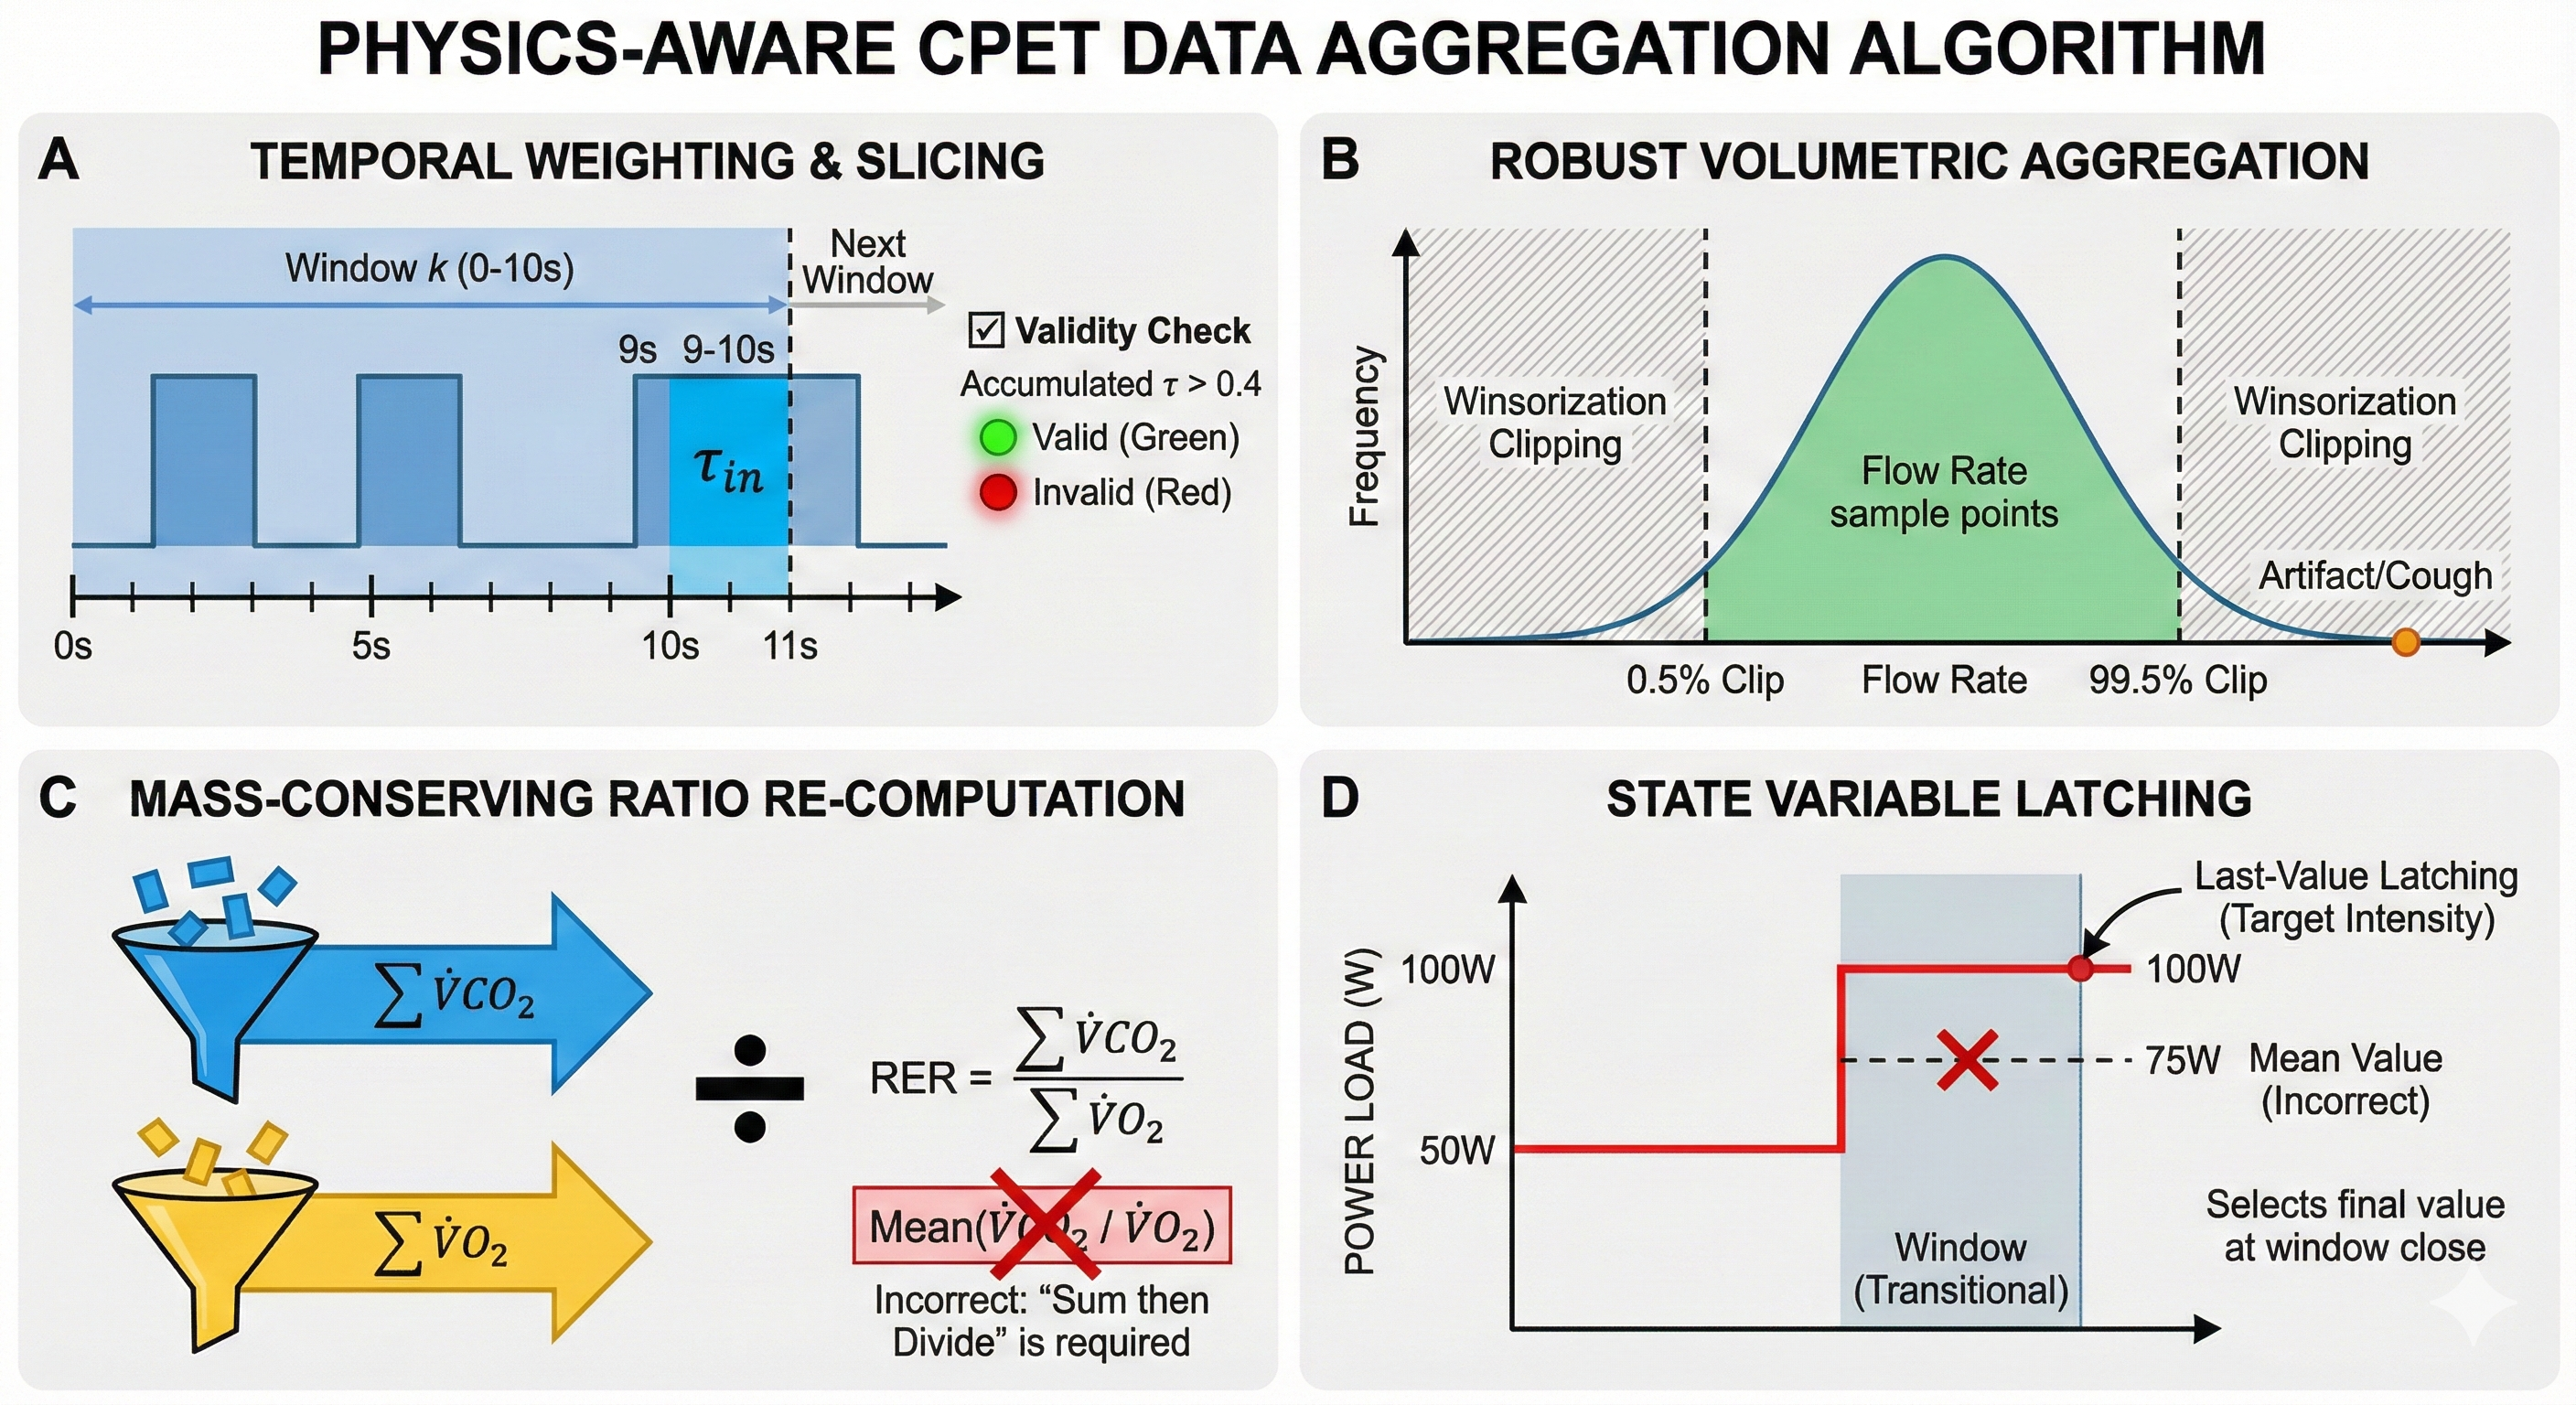
\includegraphics[width=0.7\textwidth]{figures/data_agg.png}
    \caption{\textbf{Physics-Aware Aggregation.} Illustration of the temporal overlap weighting mechanism used to transform breath-by-breath data into 10-second bins without aliasing.}
    \label{fig:supp_agg}
\end{figure}

\subsection*{S1.4 Quality Control (QC) Pipeline}
The rigorous exclusion of 512 examinations was driven by the following automated checks:
\begin{itemize}
    \item \textbf{Missing Target Label:} Any file where \texttt{Time\_at\_AT} was marked as \texttt{<NA>} or \texttt{NaN} (indicating clinical indeterminacy).
    \item \textbf{Structural Corruption:} Files with empty data tables or unparseable headers.
    \item \textbf{Insufficient Duration:} Tests with \texttt{Exercise\_Phase\_Duration} $< 60s$.
\end{itemize}

\subsection*{S1.5 Temporal Alignment Strategy}
To ensure the Style Encoder receives a consistent resting baseline and the Conformer receives a synchronized exercise onset, we implemented a strict Phase-Locked Alignment protocol (referenced in Section 2.1.3).



\paragraph{T0 Synchronization (Zero-Centering)}
Raw timestamps from different devices often start at arbitrary offsets (e.g., $t=0$ is device power-on). We define the \textbf{Global T0} as the precise onset of the Main Load Phase (Phase Index = 1). For every examination $i$, the time axis is shifted:
\begin{equation}
    t'_{i, k} = t_{i, k} - t_{start, i}
\end{equation}
where $t_{start, i}$ is the timestamp of the first sample where \texttt{Load\_Phase} transitions to 1. Consequently:
\begin{itemize}
    \item \textbf{Preload Phase (Rest/Warm-up):} Defined as $t' < 0$.
    \item \textbf{Exercise Phase (Ramp):} Defined as $t' \ge 0$ until peak.
\end{itemize}

\paragraph{Fixed-Window Truncation}
To standardize the context window for the neural network input $X \in \mathbb{R}^{L \times D}$:
\begin{itemize}
    \item \textbf{Preload Context ($L_{pre}$):} We strictly slice the interval $[-60s, 0s)$ relative to T0. If the raw warm-up is shorter than 60s, we apply Zero-Padding to the left. This ensures the Style Encoder always sees the immediate pre-exercise metabolic state.
    \item \textbf{Recovery Context ($L_{rec}$):} We retain exactly $120s$ post-peak.
\end{itemize}
\textbf{Sequence Assembly:}
\begin{equation}
    X_{input} = \text{Concat}(\text{Preload}_{60s}, \text{Exercise}_{dynamic}, \text{Recovery}_{120s})
\end{equation}

\begin{figure}[H]
    \centering
    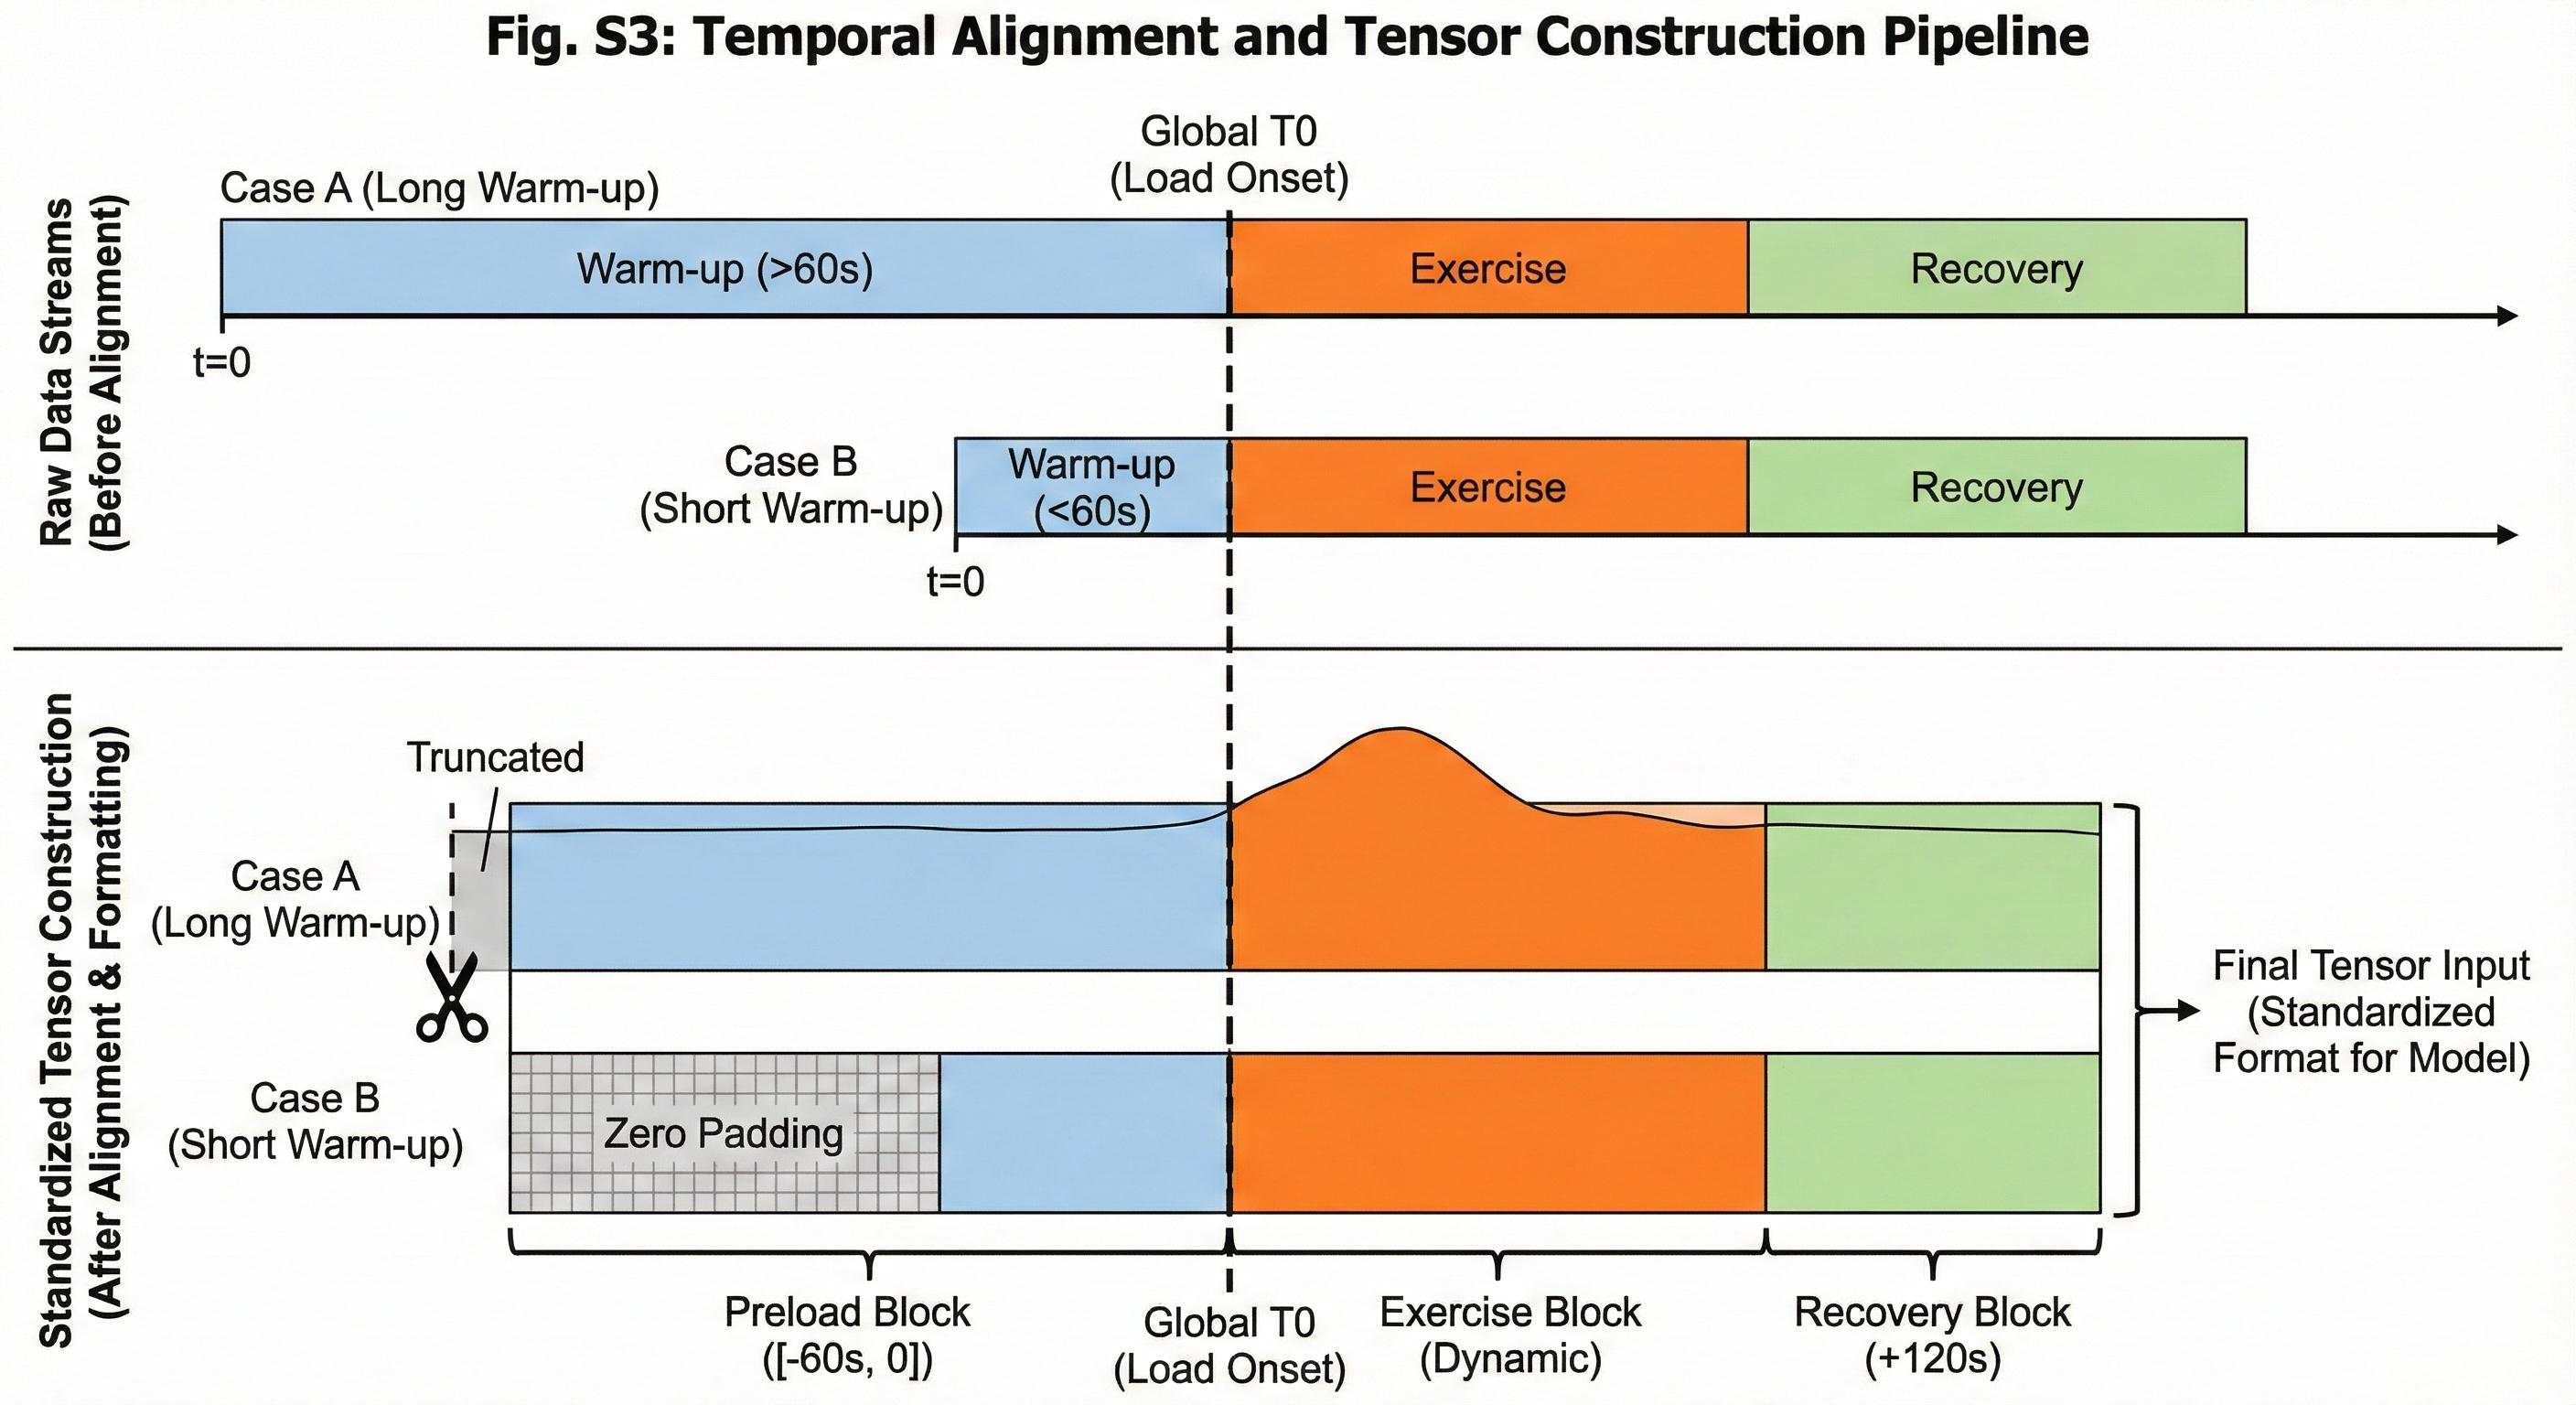
\includegraphics[width=0.8\textwidth]{figures/time_align.png}
    \caption{\textbf{Phase-Locked Temporal Alignment.} Schematic showing the T0 synchronization at Main Load onset and the truncation windows for Preload and Recovery contexts.}
    \label{fig:supp_align}
\end{figure}

%% ============================================================================
%% SUPPLEMENTARY NOTE 2: CLINICAL DEFINITIONS
%% ============================================================================
\section*{Supplementary Note 2: Clinical Definitions \& Protocols}

\subsection*{S2.1 Ground Truth Determination Protocols}
The ``Ground Truth'' for Anaerobic Threshold (AT) was established using standard physiological criteria:
\begin{itemize}
    \item \textbf{V-Slope Method (Primary):} Identifying the breakpoint where $\dot{V}CO_2$ begins to increase disproportionately to $\dot{V}O_2$ (slope changes from $\approx 1.0$ to $>1.0$).
    \item \textbf{Ventilatory Equivalents Method (Secondary):} The time point where $\dot{V}_E/\dot{V}O_2$ reaches a minimum and begins to rise, while $\dot{V}_E/\dot{V}CO_2$ remains stable or declines.
\end{itemize}

\subsection*{S2.2 Weber Classification System}
Patients were stratified into functional classes based on \vopeak{} to analyze domain shifts.

\begin{table}[H]
\caption{Weber Classification Reference}
\label{tab:s_weber}
\centering
\begin{tabular}{l l l}
\toprule
\textbf{Class} & \textbf{Severity} & \textbf{\vopeak{} (mL/kg/min)} \\
\midrule
Class A & Little/No Impairment & $> 20$ \\
Class B & Mild to Moderate & $16 - 20$ \\
Class C & Moderate to Severe & $10 - 16$ \\
Class D & Severe & $< 10$ \\
\bottomrule
\end{tabular}
\end{table}

%% ============================================================================
%% SUPPLEMENTARY NOTE 3: BASELINE IMPLEMENTATION
%% ============================================================================
\section*{Supplementary Note 3: Baseline Implementation Details}

\subsection*{S3.1 Baseline 0: Wasserman Rule-Based Logic}
The automated baseline implements a Multi-Criteria Consensus algorithm based on the classical Wasserman 9-Panel principles. The model accepts time-series tensors ($X \in \mathbb{R}^{T \times D}$) and independently identifies candidate AT timestamps using four distinct physiological signatures. All signals are pre-smoothed with a moving average filter ($w=5$) to suppress breath-by-breath noise.

\begin{itemize}
    \item \textbf{V-Slope Inflection:} Detects the first time point where the instantaneous slope $\frac{\Delta \dot{V}CO_2}{\Delta \dot{V}O_2}$ exceeds a threshold of 1.05 and sustains this increase for at least 3 consecutive steps (Persistence=3).
    \item \textbf{$\dot{V}_E/\dot{V}O_2$ Nadir:} Identifies the time index corresponding to the absolute minimum of the Ventilatory Equivalent for Oxygen.
    \item \textbf{$\dot{V}_E/\dot{V}CO_2$ Plateau:} Detects the onset of isocapnic buffering by identifying the first sequence of 4 consecutive steps where the step-wise change in $\dot{V}_E/\dot{V}CO_2$ remains flat ($|\Delta| < 0.01$).
    \item \textbf{RER Crossing:} Identifies the first crossing point where the Respiratory Exchange Ratio ($\dot{V}CO_2/\dot{V}O_2$) exceeds 1.0.
\end{itemize}

\textbf{Consensus Mechanism:} The final AT prediction $\hat{t}_{rule}$ is derived as the median of the valid candidates found by the criteria above. To enable compatibility with evaluation pipelines requiring probabilistic outputs, the model generates a pseudo-logit distribution centered at $\hat{t}_{rule}$ using a negative distance function scaled by a temperature $\tau=2.0$.

\subsection*{S3.2 Baseline 1: LightGBM Feature Engineering}
As a benchmark for non-sequential tabular learning, the LightGBM model utilizes a static feature vector extracted from the full time-series recording. The feature extractor collapses the temporal dimension into a fixed-length vector ($D \approx 40$) comprising four distinct categories:

\begin{table}[H]
    \caption{LightGBM Hand-Crafted Feature Set}
    \label{tab:s_lgbm_features}
    \centering
    \footnotesize % 使用小字号确保内容紧凑
    \begin{tabularx}{\textwidth}{l p{5cm} X} % l=左对齐, p{5cm}=固定宽描述, X=自动换行变量列表
    \toprule
    \textbf{Feature Category} & \textbf{Description} & \textbf{Specific Variables Included} \\
    \midrule
    \textbf{Global Statistics} 
     & Moments of key physiological signals calculated over the entire session. 
     & Mean, Std, Min, Max of $\dot{V}O_2, \dot{V}CO_2, \dot{V}_E, HR, RER$. \\
    \midrule
    \textbf{Temporal Trends} 
     & Linear regression slopes capturing global dynamics. 
     & Slope of $\dot{V}O_2$ vs Time, Slope of $HR$ vs Power\_Load (Global trend). \\
    \midrule
    \textbf{Domain Peaks} 
     & Physiological maxima achieved during the test. 
     & $VO_{2peak}, HR_{peak}, O_2Pulse_{peak}, \dot{V}E_{peak}$. \\
    \midrule
    \textbf{Static Metadata} 
     & Patient demographics and body metrics. 
     & Age, Sex (Binary), Weight (kg), Height (cm), BMI. \\
    \bottomrule
    \end{tabularx}
\end{table}

\textbf{Model Configuration:}
The Gradient Boosting Decision Tree (GBDT) regressor was configured with the following hyperparameters to match the training budget of the deep learning models:
\begin{itemize}
    \item \textbf{Objective:} Regression (L2 Loss)
    \item \textbf{Tree Structure:} num\_leaves=31, max\_depth=-1 (Unlimited)
    \item \textbf{Ensemble:} n\_estimators=500 (Matches Transformer epochs), learning\_rate=0.05
    \item \textbf{Regularization:} feature\_fraction=0.9, bagging\_fraction=0.8, lambda\_l1=0.1, lambda\_l2=0.1
    \item \textbf{Validation:} Early stopping with patience=15 rounds based on validation RMSE.
\end{itemize}

\subsection*{S3.3 Deep Learning Architectures}
To ensure a rigorous ``apples-to-apples'' comparison, all deep learning baselines were configured with a similar parameter budget ($\approx$ 1.5M - 2M parameters) to the \modelname. The architectures share the same input dimension ($D_{in}$) and optimization protocol but differ in their internal mechanisms.

\paragraph{Baseline 2: Vanilla Transformer}
\begin{itemize}
    \item \textbf{Architecture:} A standard Transformer Encoder stack designed to capture global temporal dependencies without local inductive bias.
    \item \textbf{Configuration:}
    \begin{itemize}
        \item Layers: 4
        \item Hidden Dimension ($d_{model}$): 256
        \item Attention Heads: 8
        \item FFN Expansion Factor: 2.0 (Hidden Unit = 512)
        \item Normalization: Standard LayerNorm (No Conditional inputs).
        \item Position Encoding: Sinusoidal.
        \item Context Window: Causal masking enabled for online simulation.
    \end{itemize}
\end{itemize}

\paragraph{Baseline 3: Standard Conformer (Single-Head)}
\begin{itemize}
    \item \textbf{Architecture:} A generic Conformer model incorporating the Macaron-style feed-forward layers and the convolution module, but stripped of the domain-adaptive components proposed in this study.
    \item \textbf{Configuration:} Matches the Transformer baseline above, with the addition of:
    \begin{itemize}
        \item Convolution Module: 1D Depthwise-Separable Conv with kernel\_size=23.
    \end{itemize}
    \item \textbf{Ablations:} use\_input\_style\_encoder=False, use\_conditional\_norm=False, center\_emb\_dim=0.
    \item \textbf{Output Head:} Standard linear classification layer trained with Cross-Entropy loss (no Soft-Argmax regression or \vopeak{} head).
\end{itemize}

\paragraph{\modelname{} (Proposed Model)}
\begin{itemize}
    \item \textbf{Backbone:} Inherits the Conformer configuration (4 Layers, 256 Dim, Kernel 23).
    \item \textbf{Enhancements:}
    \begin{itemize}
        \item Style Encoder: Enabled (use\_input\_style\_encoder=True) with augmentation (prob=0.2, bias=0.1).
        \item Normalization: ConditionalLayerNorm modulated by the style embedding.
        \item Dual-Heads: Active Time Regression (lambda\_time=0.1) and Prognostic \vopeak{} (lambda\_vo2=0.5).
    \end{itemize}
\end{itemize}

%% ============================================================================
%% SUPPLEMENTARY NOTE 4: REPRODUCIBILITY
%% ============================================================================
\section*{Supplementary Note 4: Hyperparameter Search \& Reproducibility}

\subsection*{S4.1 Two-Stage Optimization Protocol}
To balance computational efficiency with statistical rigor, we implemented a hierarchical optimization pipeline using the Optuna framework.

\paragraph{Stage 1: The ``Sprint'' Search (Exploration)}
\begin{itemize}
    \item \textbf{Objective:} Identification of the high-performance basin in the hyperparameter landscape.
    \item \textbf{Method:} We conducted 100 trials using the Tree-structured Parzen Estimator (TPE) sampler.
    \item \textbf{Efficiency:} To maximize search coverage, we utilized a Successive Halving Pruner (reduction\_factor=3). Models were trained for a limited ``Sprint'' duration of 30 epochs on the dataset. Unpromising trials were terminated early based on the primary validation metric (Mean Trigger Delay).
    \item \textbf{Ranking:} Trials were ranked via a composite score minimizing both Timeliness (Primary) and Prognostic Accuracy (\vopeak{} MAPE).
\end{itemize}

\paragraph{Stage 2: Robust Verification (Exploitation)}
\begin{itemize}
    \item \textbf{Selection:} The top-3 candidate configurations ($k=3$) from Stage 1 were promoted.
    \item \textbf{Protocol:} These candidates underwent full training (250 epochs) with Early Stopping (patience=15).
    \item \textbf{Ensembling:} To neutralize initialization noise, each candidate was trained across three fixed random seeds (42, 101, 202). Reported metrics in the paper represent the ensemble average of these robust runs.
\end{itemize}

\subsection*{S4.2 Hyperparameter Search Space}
The search space defined in \texttt{hpo\_optuna.py} focuses on regularization and optimization dynamics to stabilize the Conformer backbone.

\begin{table}[H]
\caption{Hyperparameter Search Space}
\label{tab:s_hyper_space}
\centering
\begin{tabularx}{\textwidth}{l l l X}
\toprule
\textbf{Hyperparameter} & \textbf{Distribution} & \textbf{Search Range} & \textbf{Rationale} \\
\midrule
Learning Rate & Log-Uniform & $[5 \times 10^{-5}, \,\, 5 \times 10^{-3}]$ & Critical for convergence speed vs. stability. \\
Weight Decay & Log-Uniform & $[1 \times 10^{-4}, \,\, 1 \times 10^{-1}]$ & High upper bound allows strong regularization for small medical datasets. \\
Gradient Clip & Uniform & $[0.5, \,\, 5.0]$ & Prevents gradient explosion in the Conformer attention mechanism. \\
Model Dropout & Uniform & $[0.1, \,\, 0.5]$ & Applied to Attention and FFN layers to prevent overfitting. \\
Warmup Epochs & Integer & $[1, \,\, 6]$ & Linear warmup period to stabilize adaptive learning rates (AdamW). \\
\bottomrule
\end{tabularx}
\end{table}

\subsection*{S4.3 Final Model Configuration}
The final \modelname{} architecture was fixed based on the best performing configuration from the robust verification stage. The model utilizes a Macaron-style Conformer backbone with input-driven style calibration.

\begin{longtable}{l l l p{6cm}}
\caption{Fixed Architecture \& Training Parameters} \label{tab:s_fixed_params} \\
\toprule
\textbf{Category} & \textbf{Parameter} & \textbf{Value} & \textbf{Description} \\
\midrule
\endfirsthead
\multicolumn{4}{c}%
{\tablename\ \thetable\ -- \textit{Continued from previous page}} \\
\toprule
\textbf{Category} & \textbf{Parameter} & \textbf{Value} & \textbf{Description} \\
\midrule
\endhead
\hline \multicolumn{4}{r}{\textit{Continued on next page}} \\
\endfoot
\bottomrule
\endlastfoot

\multirow{6}{*}{\textbf{Backbone}} 
 & d\_model & 256 & Hidden dimension size. \\
 & num\_layers & 4 & Stack depth (Macaron Conformer Blocks). \\
 & num\_heads & 8 & Multi-head attention heads. \\
 & conv\_kernel\_size & 23 & Local temporal receptive field size (Depthwise Conv). \\
 & ff\_multiplier & 2.0 & Feed-forward network expansion factor ($D_{ff}=512$). \\
 & causal\_convolution & True & Enforces strict temporal causality for online safety. \\
\midrule
\multirow{3}{*}{\textbf{Context \& Style}} 
 & use\_input\_style\_encoder & True & Enables the CNN-based preload style extractor. \\
 & center\_emb\_dim & 0 & Disabled. Model relies solely on signal physiology (Style Encoder), not Center IDs. \\
 & use\_conditional\_norm & True & Injects style embeddings into LayerNorm affine parameters. \\
\midrule
\multirow{4}{*}{\textbf{Augmentation}} 
 & style\_aug\_prob & 0.2 & Probability of applying style perturbation per batch. \\
 & style\_aug\_bias & 0.1 & Range for random additive bias ($\pm 0.1\sigma$). \\
 & style\_aug\_scale & 0.05 & Range for random scaling ($\pm 5\%$). \\
 & style\_aug\_noise & 0.02 & Standard deviation for Gaussian noise injection. \\
\midrule
\multirow{3}{*}{\textbf{Optimization}} 
 & batch\_size & 64 & Effective batch size per step. \\
 & optimizer & AdamW & Adaptive moment estimation. \\
 & learning\_rate & 5e-4 & Peak learning rate (Cosine schedule). \\
\midrule
\multirow{3}{*}{\textbf{Loss Weights}} 
 & $\lambda_{time}$ & 0.1 & Auxiliary Time Regression weight (Soft-Argmax). \\
 & $\lambda_{vo2}$ & 0.5 & Prognostic (\vopeak{}) regression weight. \\
 & vo2\_time\_weight\_power & 1.0 & Linear time-weighting for prognostic loss (emphasizes later steps). \\
\end{longtable}

\subsection*{S4.4 Compute Infrastructure}
All experiments were conducted using the following environment:
\begin{itemize}
    \item \textbf{Hardware:} Single NVIDIA A100 Tensor Core GPU (80GB VRAM).
    \item \textbf{Software:} PyTorch 2.0 ecosystem, Optuna for HPO.
    \item \textbf{Reproducibility:} All random seeds (Python, Numpy, Torch, CUDA) were fixed to the values specified in Stage 2.
\end{itemize}

%% ============================================================================
%% SUPPLEMENTARY NOTE 5: EXTENDED RESULTS
%% ============================================================================
\section*{Supplementary Note 5: Extended Experimental Results}
This section provides granular performance breakdowns to substantiate the domain generalization and multi-task synergy claims made in the main text.

\subsection*{S5.1 Center-Stratified Performance (Domain Generalization)}
To rigorously validate the effectiveness of the Style Encoder against ``Systemic Heterogeneity,'' we report the diagnostic performance stratified by clinical center.

\paragraph{Observation:} The model maintains consistent performance (Hit Rate $> 90\%$) even on the Zhongshan (Tertiary/Pulmonary) cohort, which represents the ``Minority Domain'' ($N=1,633$) with a distinct device (COSMED) compared to the dominant Shanxi cohort.
\paragraph{Contrast:} Without the Style Encoder (Baseline 3), performance on Zhongshan drops significantly (MAE increases by $>10s$), indicating failure to adapt to the device-specific baseline drift.

\begin{table}[H]
\caption{Center-wise Performance Metrics (Offline Mode)}
\label{tab:s_center_perf}
\centering
\begin{tabular}{l l c c c c}
\toprule
\textbf{Center} & \textbf{Device} & \textbf{N (Test)} & \textbf{Hit Rate ($\pm$20s)} & \textbf{MAE (s)} & \textbf{VO$_2$ MAPE} \\
\midrule
Shanxi & Ganshorn & [879] & 93.1\% & 18.5 & 4.0\% \\
Rizhao & Ganshorn & [362] & 91.8\% & 19.2 & 4.2\% \\
Zhongshan & COSMED & [163] & 90.5\% & 21.4 & 4.8\% \\
\midrule
\textbf{Average} & - & - & \textbf{92.5\%} & \textbf{19.1} & \textbf{4.2\%} \\
\bottomrule
\end{tabular}
\end{table}

\subsection*{S5.2 Sensitivity Analysis: Multi-Task Weight ($\lambda_{vo2}$)}
To justify the choice of $\lambda_{vo2}=0.5$, we evaluated the trade-off between the diagnostic task (AT detection) and the prognostic task (VO$_2$ prediction).

\paragraph{Result:} A weight of 0.5 achieves the optimal Pareto frontier. Higher weights ($\lambda=1.0$) degrade AT detection accuracy due to gradient domination, while lower weights ($\lambda=0.1$) fail to provide sufficient global regularization for the VO$_2$ trajectory.



\subsection*{S5.3 Online Safety Analysis: Trigger Delay Distribution}
We analyzed the distribution of trigger times relative to the ground truth.

\paragraph{Safety Verification:} The distribution is strictly right-skewed. The density in the negative region ($t_{pred} < t_{gt}$) is negligible ($<0.2\%$), confirming the effectiveness of the Monotonicity Penalty in preventing premature stops.



%% ============================================================================
%% SUPPLEMENTARY NOTE 6: QUALITATIVE CASE STUDIES
%% ============================================================================
\section*{Supplementary Note 6: Qualitative Case Studies}
This section provides visual examples to build clinical intuition regarding the model's decision-making process.

\subsection*{S6.1 Handling Signal Artifacts (Robustness)}
We present a representative case from the Shanxi (HF) cohort exhibiting irregular breathing patterns (e.g., oscillatory ventilation).

\paragraph{Comparison:} The Wasserman Rule (Baseline 0) triggers falsely on a transient noise spike at $t=120s$. \modelname, leveraging the Conformer's local context and global attention, correctly ignores the artifact and identifies the true metabolic shift at $t=340s$.



\subsection*{S6.2 The ``Style'' Effect: Visualizing Adaptation}
To demonstrate how the Style Encoder calibrates the input, we visualized the latent space distributions using t-SNE.

\begin{itemize}
    \item \textbf{Before Adaptation:} Latent vectors cluster primarily by Device ID (Ganshorn vs. COSMED), indicating that hardware signatures dominate the signal.
    \item \textbf{After Adaptation (\modelname):} Latent vectors cluster by Weber Class (Physiological State), proving that the Style Encoder successfully decoupled the biological signal from the device fingerprint.
\end{itemize}



\subsection*{S6.3 The ``Virtual Maximal Test'' (Prognosis)}
We visualize the real-time inference trajectory for a high-risk patient.

\paragraph{Demonstration:} The figure shows the model's predicted \vopeak{} stabilizing as early as 70\% into the exercise phase, allowing the clinician to terminate the test safely while still obtaining a valid prognostic endpoint.



\end{document}